\documentclass[12pt,a4paper]{report}

% ======================================================
% IDIOMA E CODIFICAÇÃO
% ======================================================
% Idioma PT-BR e hifenização correta
\usepackage[brazil]{babel}

% Codificação de fontes (necessária mesmo com fontspec em alguns casos)
\usepackage[T1]{fontenc}

% ======================================================
% FONTES (XeLaTeX / LuaLaTeX)
% ======================================================
% Permite usar fontes do sistema
\usepackage{fontspec}
\setmainfont{Montserrat}
\usepackage{indentfirst}


% ======================================================
% LAYOUT DE PÁGINA
% ======================================================
\usepackage{geometry}
\geometry{
  left=3cm,
  right=2cm,
  top=2.5cm,
  bottom=3cm
}

\setlength{\footskip}{2cm}

% Remove bordas do hyperlink no sumário
\usepackage{hyperref}
\hypersetup{
  pdfborder={0 0 0}
}

% Espaçamento entre linhas
\usepackage{setspace}
\onehalfspacing

% Parágrafo
\setlength{\parindent}{1.5cm}
\setlength{\parskip}{0.5em}

\newcommand{\capaCustomizada}{
\RodapeAtivofalse % <<< DESLIGA RODAPÉ
\begin{titlepage}
\thispagestyle{empty}


% ======================
% TOPO (imagem cabeca.png) – centralizada e menor
% ======================
\begin{tikzpicture}[remember picture,overlay]
\node[
  anchor=north,
  inner sep=0pt
] 
at ([yshift=-1cm]current page.north)
{
\includegraphics[width=0.9\paperwidth]{cabeca.png}};
\end{tikzpicture}

% ======================
% CONTEÚDO CENTRAL
% ======================
\begin{tikzpicture}[remember picture,overlay]

% TÍTULO PRINCIPAL
\node[
  anchor=west,
  font=\bfseries\fontsize{24pt}{28pt}\selectfont,
  text=black
]
at ([xshift=3cm,yshift=-10cm]current page.north west)
{Relatório Maturidade};

% SUBTÍTULO
\node[
  anchor=west,
  font=\fontsize{14pt}{18pt}\selectfont,
  text=black
]
at ([xshift=3cm,yshift=-11.2cm]current page.north west)
{Processo de Qualidade de Software};

% Logo TC capa
\node[
  anchor=west
]
at ([xshift=14.5cm,yshift=-10.6cm]current page.north west)
{
\includegraphics[height=2cm]{icone.png}};


\end{tikzpicture}

% ======================
% RODAPÉ PRETO
% ======================
\AddToShipoutPictureBG*{
  \AtPageLowerLeft{
\begin{tikzpicture}[remember picture,overlay]

% Fundo preto
\fill[black]
  (current page.south west)
  rectangle
  ([yshift=3cm]current page.south east);

% Link centralizado
\node[
  anchor=south,
  text=white,
  font=\fontsize{12pt}{11pt}\selectfont
]
at ([yshift=1cm]current page.south)
{\href{https://www.testingcompany.com.br}{\centering www.testingcompany.com.br}};

\end{tikzpicture}

  }
}

\end{titlepage}
\RodapeAtivotrue % <<< RELIGA RODAPÉ
}

% ======================================================
% RODAPÉ PADRÃO (IMAGEM)
% ======================================================
\newcommand{\RodapeImagem}{%
  \AddToShipoutPictureBG*{%
    \AtPageLowerLeft{%
      
\includegraphics[
        width=\paperwidth
      ]{rodape.png}%
    }%
  }%
}



% ======================================================
% CORES E IMAGENS
% ======================================================
\usepackage{xcolor}
\usepackage{graphicx}
\usepackage{float}

% Fundo usado em páginas de abertura de capítulo
\newcommand{\ChapterBackground}{%
  \AddToShipoutPictureBG*{%
    \AtPageUpperLeft{%
      \raisebox{-\paperheight}{%
        
\includegraphics[
          width=\paperwidth,
          height=\paperheight
        ]{fundo_titulo}%
      }%
    }%
  }%
}

\newcommand{\PaginaFinalImagem}[1]{%
  \clearpage
  \RodapeAtivofalse % desliga rodapé
  \thispagestyle{empty}

  \begin{tikzpicture}[remember picture,overlay]
    \node[
      anchor=center
    ] at (current page.center)
    {\includegraphics[
      width=\paperwidth,
      height=\paperheight
    ]{#1}};
  \end{tikzpicture}

  \clearpage
  \RodapeAtivotrue % religa rodapé (se houver páginas depois)
}




% ======================================================
% TÍTULOS E ESTRUTURA
% ======================================================
% Customização de títulos (chapter, section, subsection)
\usepackage{titlesec}

% --- REMOVE QUALQUER NUMERAÇÃO VISUAL DO CHAPTER ---
% Mantém contador e TOC, mas impede o "1" de aparecer
\makeatletter
\renewcommand{\@makechapterhead}[1]{%
  \vspace*{50pt}%
  {\parindent \z@ \raggedright
    \normalfont
    \Huge\mdseries
    #1\par\nobreak
    \vskip 40pt
  }}
\renewcommand{\@makeschapterhead}{\@makechapterhead}
\newcommand{\ChapterFont}{\fontsize{20pt}{26pt}\selectfont}
\newcommand{\SectionFont}{\fontsize{16pt}{6pt}\selectfont}
\newcommand{\SubSectionFont}{\fontsize{14pt}{6pt}\selectfont}
\makeatother

% Formato visual do CHAPTER (somente ícone, sem título duplicado)
\titleformat{name=\chapter}
  {\ChapterFont\color{black}}
  {}
  {0pt}
  {
\includegraphics[height=0.9em]{icone.png}\hspace{0.5em}}

% Seções
\titleformat{\section}
  {\SectionFont\color{red}}
  {\hspace{1.5em}\thesection}
  {1em}
  {}

\titleformat{\subsection}
  {\SubSectionFont\color{red}}
  {\hspace{4em}\thesubsection}
  {1em}
  {}

% Profundidade de numeração e sumário
\setcounter{tocdepth}{3}
\setcounter{secnumdepth}{3}

% ======================================================
% FUNDO DE PÁGINA (SPECIAL CHAPTER)
% ======================================================
%\usepackage{background}
\usepackage{eso-pic}
\usepackage{etoolbox}

\newif\ifChapterBackgroundEnabled
\ChapterBackgroundEnabledtrue


% ======================================================
% APLICA FUNDO AUTOMÁTICO EM TODOS OS CHAPTERS NORMAIS
% ======================================================
\makeatletter
\pretocmd{\chapter}{%
  \clearpage
  \thispagestyle{empty}
  \ifChapterBackgroundEnabled
    \ChapterBackground
  \fi
}{}{}
\makeatother



% ======================================================
% TIKZ (LAYOUT ABSOLUTO DOS TÍTULOS ESPECIAIS)
% ======================================================
\usepackage{tikz}
\usetikzlibrary{calc}

% ======================================================
% CAPÍTULO ESPECIAL (LAYOUT PRÓPRIO)
% ======================================================
\newcommand{\specialchapter}[2]{%
  \clearpage
  \thispagestyle{empty}

  % Contador + TOC
  \refstepcounter{chapter}
  \addcontentsline{toc}{chapter}{\thechapter\quad #1}

% DESLIGA FUNDO NORMAL
\ChapterBackgroundEnabledfalse

% FUNDO ESPELHADO HORIZONTAL
\AddToShipoutPictureBG*{%
  \AtPageLowerLeft{%
    \reflectbox{%
      
\includegraphics[
        width=\paperwidth,
        height=\paperheight
      ]{fundo_titulo}%
    }%
  }%
}
% LIMPA FUNDO PARA NÃO VAZAR
\ClearShipoutPictureBG
\ChapterBackgroundEnabledtrue
\clearpage

  % =========================
  % CONTEÚDO
  % =========================
  \begin{tikzpicture}[remember picture,overlay]

    % Título
    \node[
      anchor=west,
      font=\Huge,
      text=black
    ]
    at ([xshift=8cm,yshift=-8cm]current page.north west)
    {#1\hspace{0.5em}
\includegraphics[height=0.9em]{icone.png}};

    % Caixa preta
    \node[
      anchor=north west,
      fill=black,
      text=white,
      inner sep=1.2cm,
      text width=0.50\paperwidth,
      align=justify
    ]
    at ([xshift=8cm,yshift=-9cm]current page.north west)
    {#2};

  \end{tikzpicture}

  % LIMPA FUNDO PARA NÃO VAZAR
  \ClearShipoutPictureBG
  \clearpage
}

%impede o vazamento do rodapé
\newif\ifRodapeAtivo
\RodapeAtivotrue


% Aplica rodapé em todas as páginas
\AddToHook{shipout/foreground}{%
  \ifRodapeAtivo
    \begin{tikzpicture}[remember picture,overlay]
      \node[
        anchor=south west,
        xshift=-0.01\paperwidth,
        opacity=0.5
      ] at (current page.south west)
      {\scalebox{1.05}[1]{%
        
\includegraphics[width=\paperwidth]{rodape.png}%
      }};
    \end{tikzpicture}
  \fi
}




% ======================================================
% UTILITÁRIOS
% ======================================================
\usepackage{hyperref}
\usepackage{longtable}
\usepackage{caption}

% =========================
% Final do Preâmbulo 
% =========================
% Dados do documento
% =========================
\title{Relatório de Maturidade\\Processo de Qualidade de Software}
\author{Testing Company}
\date{\today}



\begin{document}

\capaCustomizada
\tableofcontents
\newpage

% =========================
% Introdução
% =========================
    \chapter{Introdução}

O presente relatório tem como objetivo principal expor a avaliação dos processos iniciada a partir da aprovação do projeto de escopo fechado entre a Testing Company e a ALS Global. A organização contratante reconhece que seu sistema atualmente possui zero teste e a concentração dos problemas estão nas melhorias realizadas nos anos anteriores. Assim, é interessante que seja avaliado um processo de teste que apoie a identificar incidentes antes que os mesmos cheguem em ambiente produtivo. 

As atividades da equipe da Testing Company, apoiadas em conversas com os profissionais da empresa, foram conduzidas inicialmente no entendimento do sistema, processos, problemas e oportunidades de melhora dentro da organização. Sendo assim, a avaliação de maturidade indica o estágio em que os processos se encontram utilizando a jornada da qualidade da Testing Company. Este plano baseia-se no modelo de maturidade com cinco níveis distintos que indicam o alinhamento da organização com o modelo de referência.

A estrutura é dividida em estágios, começando pelo nível inicial que se caracteriza-se por ser a etapa em que os testes são definidos de acordo com a intuição, possui ausência de automação, mas já existe documentação de defeitos identificados. O modelo segue até o nível cinco, denominado de otimizado, que se caracteriza pelos poucos defeitos encontrados em ambiente produtivo, possuindo métricas que retroalimentam o processo de qualidade, testes automatizados presentes em pipelines e entre outros. 

O relatório está estruturado em 7 capítulos, dos quais são descritos o plano de trabalho aplicado ao longo do andamento do projeto juntamente com explicações teóricas para embasar assuntos técnicos e processuais utilizados. Não é o objetivo propor diretamente soluções para eventuais problemas identificados neste momento, entretanto alguns deles podem ser expostos ao longo do documento. 


% =========================
% Objetivo
% =========================
\specialchapter
{Objetivo}
{
Este relatório apresenta aspectos da avaliação de maturidade dos processos de qualidade de software da ALS Global, realizada pela Testing Company. A análise irá diagnosticar o estágio atual dos processos, identificando pontos de evolução e possíveis melhorias. Para isso, será comentado o plano de trabalho aplicado, bem como os alguns pontos relacionados a avaliação. Embora o foco do documento não seja propor soluções diretas, eventuais problemas e oportunidades de aprimoramento podem ser destacados.
}

% =========================
% Planejamento Inicial
% =========================
\chapter{Planejamento Inicial}

\section{Escopo do Projeto}

O escopo de trabalho em sua totalidade está atrelado ao diagnóstico e proposta de melhoria da qualidade na empresa contratante, englobando Assessment e Plano da Qualidade. Algumas das atividades realizadas, em um primeiro momento, estão focadas no entendimento e conhecimento da situação atual em que a ALS Global se encontra. O escopo contempla duas etapas. As fases iniciais pertencentes a etapa de Assessment envolvem a contextualização, na qual profissionais da Testing Company compreendem alguns aspectos do funcionamento interno da empresa contratante, interagindo com colaboradores operacionais e estratégicos.



\section{Fases de Atuação}

\subsection{Contextualização}

Neste momento inicial, foi realizado em conversa que, dentre alguns tópicos, abordou o produto, os processos já estabelecidos, as complexidades técnicas que permeiam o fluxo de trabalho atual, expectativas e oportunidades de melhoria. Alguns dos pontos de melhoria e dores coletados na fase de contextualização são categorizados em três aspectos diferentes da empresa (produto, processos e negócio). Vale ressaltar que o processo de entendimento contou com o apoio da equipe interna da empresa e foi conduzido por profissionais com conhecimento em qualidade de software. 

\subsection{Entrevistas e Questionários}

Com um entendimento inicial do contexto da organização, iniciou-se a adaptação e aplicação de questionários para levantar aspectos profissionais e organizacionais, por meio de um conjunto de perguntas pré-definidos. As perguntas foram aplicadas a profissionais internos e externos. Além da aplicação dos questionários, foi realizado um conjunto de entrevistas.

\subsection{Material de Assessment}

Os artefatos gerados através das fases anteriores, após compilados, expõem uma visão da situação atual da organização. Essas informações são utilizadas para apoiar a construção de uma planilha de dores e o relatório de maturidade atual. O relatório é um entregável que expõem informações coletadas que podem ser úteis para a organização, como a insatisfação e sugestões de melhorias levantadas pelos próprios colaboradores, ou até mesmo as falhas de processo que ainda não são de conhecimento de todos da gestão. Adicionalmente, avalia-se a aderência da empresa a um dos níveis estabelecidos na jornada da qualidade, utilizando o modelo de referência da Testing Company


\subsection{Plano da Qualidade}

A etapa de plano da Qualidade diz respeito às atividades em que serão pensadas sugestões e propostas para atuar sobre as imperfeições e melhorias identificadas nas etapas iniciais. A estratégia de testes caracteriza-se por ser um plano de ação, nela visa-se trazer mudanças que reflitam positivamente no processo e/ou produto como, por exemplo, redução de defeitos em ambientes produtivos ou mesmo apoiar a organização dos profissionais de qualidade. Inclui-se também sugestões a longo prazo, que podem conter atividades com tempo de implementação mais alto ou até contínuo. Entende-se que as propostas servem apenas como sugestões, podendo ou não serem aplicadas, mas ao menos as mesmas podem fornecer \textit{insights} à organização referente aos pontos do atual processo que podem ou devem ser revistos.


% =========================
% Jornada da Qualidade
% =========================

\chapter{Apresentação da Jornada da Qualidade}

 A jornada da qualidade é o modelo de maturidade presente na Testing Company. A ideia é ter uma base para compreensão do estágio em que os elementos organizacionais se encontram e apoiar nas discussões sobre o que pode ser melhorado e/ou evoluído. Nos próximos tópicos do presente capítulo será esclarecido um pouco sobre cada um dos níveis do modelo.


\section{Nível Inicial}

No estágio inicial de maturidade de um processo de qualidade é comum encontrar uma quantidade significativa de defeitos sendo descobertos somente após a fase de produção. Nesse estágio, os testes são definidos com base na intuição dos testadores, sem seguir uma abordagem sistemática ou metodologias estabelecidas. Apesar desses desafios, é importante destacar que, mesmo sem um processo estruturado, existe a prática de documentar os defeitos identificados. Essa documentação serve como um registro dos problemas encontrados e pode auxiliar na comunicação e no acompanhamento das ações corretivas necessárias. 


\begin{figure}[H]
\centering
\caption{Modelo de Maturidade – Nível Inicial}
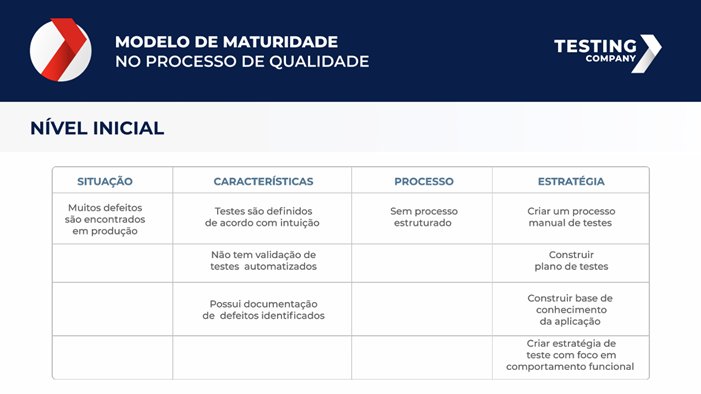
\includegraphics[width=0.7\textwidth]{inicial.png}

Fonte: Elaborado pela Testing Company
\end{figure}

\section{Nível Gerenciado}

No segundo nível de maturidade de um processo de qualidade ainda é comum encontrar uma quantidade considerável de defeitos em produção, incluindo alguns que podem ser críticos. Nesse estágio, os testes são definidos com base em uma estratégia mais estruturada, levando em consideração critérios objetivos. Embora não haja validação de testes automatizados totalmente implementados, há uma avaliação de ferramentas que possam desempenhar esse papel, incluindo a possibilidade de construir Provas de Conceito (POC). Além disso, existe a prática de documentar e monitorar os defeitos identificados. No entanto, o foco principal é garantir que o processo de qualidade esteja presente dentro do processo de desenvolvimento, priorizando a existência do processo em si, em vez de avaliar se está funcionando da maneira mais correta e eficiente possível.

\begin{figure}[H]
\centering
\caption{Modelo de Maturidade – Nível Gerenciado}
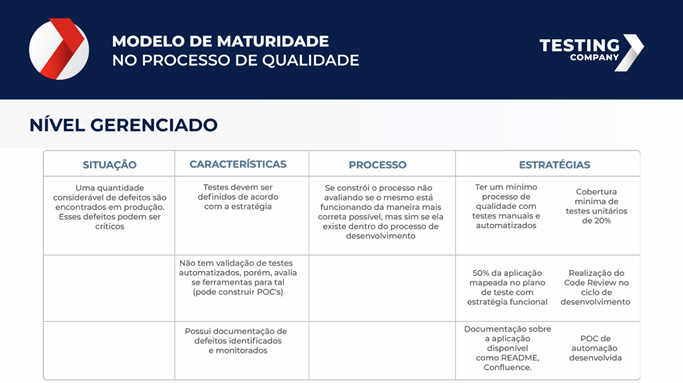
\includegraphics[width=0.7\textwidth]{gerenciado.png}

Fonte: Elaborado pela Testing Company
\end{figure}


\section{Nível Definido}

No terceiro nível de maturidade de um processo de qualidade os defeitos são detectados principalmente durante a fase de testes, resultando em uma quantidade reduzida de defeitos críticos encontrados na produção. Nesse estágio, é necessário realizar uma combinação de testes regressivos, tanto testes manuais quanto automatizados, de acordo com uma estratégia definida. Além disso, alguns testes de integração, regressão e end-to-end são automatizados para aumentar a eficiência do processo. A documentação é continuamente escrita e refinada, garantindo que esteja sempre atualizada. 

Os testes automatizados podem ser executados manualmente, permitindo maior flexibilidade e agilidade no processo. Além disso, o processo de testes manuais é executado regularmente e os testes automatizados são integrados ao processo de qualidade, garantindo uma abordagem mais abrangente e eficaz.


\begin{figure}[H]
\centering
\caption{Modelo de Maturidade – Nível Definido}
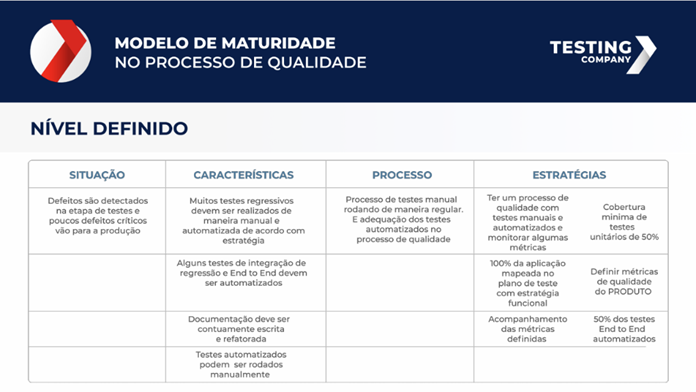
\includegraphics[width=0.7\textwidth]{definido.png}

Fonte: Elaborado pela Testing Company
\end{figure}


\section{Nível Maduro}

No quarto nível de maturidade de um processo de qualidade, é comum detectar uma quantidade significativa de defeitos durante a etapa de testes, resultando em uma quantidade mínima de defeitos que chegam à produção. Nesse estágio, a maioria dos testes regressivos é automatizada, seguindo uma estratégia bem definida, enquanto uma quantidade reduzida é realizada manualmente. 

Os testes de integração, regressão e end-to-end são amplamente automatizados para aumentar a eficiência do processo. A documentação é continuamente escrita e refinada, garantindo que esteja sempre atualizada. Parte dos testes pode ser executada manualmente ou automaticamente, dependendo da necessidade e dos recursos disponíveis. Além disso, a equipe de testes desempenha um papel ativo na estruturação dos requisitos do sistema, contribuindo para a redução de inconsistências desde o início do projeto.


\begin{figure}[H]
\centering
\caption{Modelo de Maturidade – Nível Maduro}
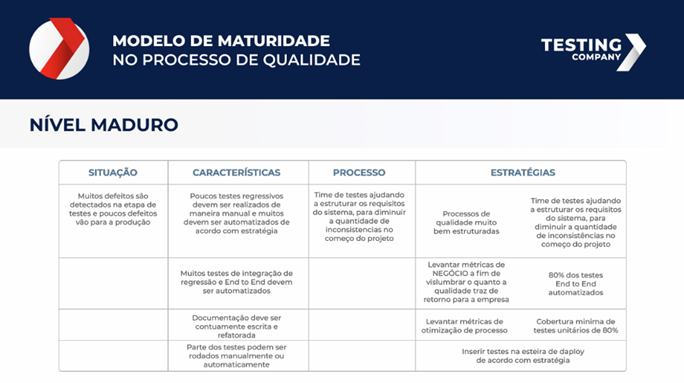
\includegraphics[width=0.7\textwidth]{maduro.png}

Fonte: Elaborado pela Testing Company
\end{figure}



\section{Nível Otimizado}

No quinto nível de maturidade de um processo de qualidade, é comum detectar a maioria dos defeitos no início do processo, antes mesmo da etapa de testes, resultando em uma quantidade mínima de defeitos críticos encontrados durante os testes e na produção. O time de qualidade desempenha um papel fundamental na disseminação da cultura de qualidade em todo o ciclo de desenvolvimento e na empresa como um todo. 

Os testes automatizados são executados automaticamente nas pipelines, otimizando o fluxo de DevOps. A documentação é gerada por meio de relatórios de automação, fornecendo informações precisas e atualizadas. Métricas são utilizadas para retroalimentar o processo de qualidade, permitindo melhorias contínuas. Os processos estão organizados e fornecem feedback sobre o produto, o processo e os aspectos de negócio, sempre buscando a melhoria contínua em todas as áreas.

\begin{figure}[H]
\centering
\caption{Modelo de Maturidade – Nível Otimizado}
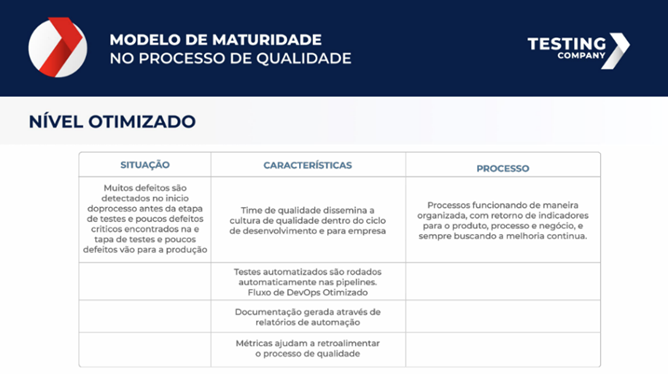
\includegraphics[width=0.7\textwidth]{otimizado.png}

Fonte: Elaborado pela Testing Company
\end{figure}


% =========================
% Análise e Diagnóstico
% =========================
\chapter{Análise e Diagnóstico Organizacional}

Iniciado o projeto, os profissionais da Testing Company foram expostos a uma visão do quadro interno geral presente na equipe. Explorando alguns aspectos como o fluxo de trabalho, juntamente com informações do produto e negócio que a empresa detém. 

É importante ressaltar que, em um primeiro momento, as interações de contextualização e conhecimento entre profissionais foram conduzida através de entrevistas e questionários. Em essência, realizou-se uma descoberta, explorando e coletando informações para apoiar os próximos passos.


\section{Metodologia de Análise}

A metodologia de análise é um guia que apoia a propor os modos com que a coleta de informações será conduzida. Para uma estratégia que visa melhoria de processo é interessante que se tenha um método de abordagem colaborativa desde as etapas iniciais. As pessoas envolvidas podem ter participado ativamente da construção e evolução do que hoje é considerado como processo da organização, sendo assim, nada mais justo do que iniciar as novas mudanças com a contribuição dos profissionais existentes.

Dessa forma, os profissionais da Testing Company se familiarizaram com o atual modo de operação. A primeira reunião para transferência de conhecimento, realizada após o início do projeto, contou com a participação de profissionais da empresa contratante, além de três profissional da área de qualidade da Testing Company. Em seguida, iniciou-se a realização de entrevistas e a elaboração de um questionário direcionado a alguns membros da equipe da empresa contratante.


\subsection{Aplicação do Questionário}

A partir das primeiras interações realizadas durante a contextualização inicial, foi definida a aplicação de dois questionários, sendo um direcionado aos colaboradores internos e outro às equipes terceiras. Em alguns casos, o questionário pode ser o único contato da consultoria com determinados colaboradores, que é o que ocorreu com alguns colaboradores terceiros, e constitui uma possibilidade para expor pontos positivos, negativos e outros aspectos relacionados ao trabalho. 

Não foi realizado entrevistas com as equipes terceiras, neste caso restringiu-se as entrevistas a cinco profissionais internos da ALS Global. Os questionários foram subdivididos em quatro seções distintas, embora não necessariamente possuem as mesmas perguntas, ou seja, as perguntas variaram entre os dois questionários. As seções dos questionários foram:

 \begin{itemize}
 	\item Dados do Profissional (Colaboradoes e Terceiros)
 	\item Fluxo de Trabalho (Colaboradoes e Terceiros) 
 	\item Teste e Qualidade (Apenas Terceiros)
 	\item Comunicação (Apenas Colaboradores)
 	\item Oportunidades de Melhoria (Apenas Terceiros)
 	\item Ferramentas (Apenas Colaboradores)
 \end{itemize}

\subsection{Realização de Conversas Individuais}

A condução de conversas individuais com alguns dos profissionais pode contemplar questões similares às levantadas nos questionários. No entanto, nesse formato, um ou mais colaboradores estão presentes durante a realização das perguntas. Uma das principais vantagens das conversas individuais é proporcionar ao profissional a oportunidade de apresentar pontos e observações adicionais, além de permitir que os entrevistadores se aprofundem em determinados assuntos.

Foram realizadas conversas com aproximadamente 4 (quatro) pessoas, pertencentes ao setor de TI. A seguir, apresenta-se uma visão geral das áreas e dos profissionais envolvidos.

\begin{figure}[H]
\centering
\caption{Tabela de Entrevistados Por Área}
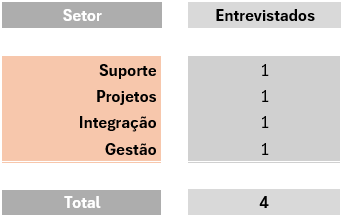
\includegraphics[width=0.7\textwidth]{entrevistados.png}

Fonte: Elaborado pela Testing Company
\end{figure}


\section{Metodologia de Categorização e Classificação de Problemas}

A metodologia de análise apresentada até o momento normalmente resulta em um grande volume de informações relacionadas à forma como o setor é conduzido, bem como aos pontos de melhoria e às principais dores identificadas. Dessa forma, a categorização e a classificação dos problemas possibilitam organizar e detalhar parte das informações obtidas na etapa anterior, contribuindo para a construção de um entregável que consolida alguns dos problemas e pontos de melhoria relatados pelos profissionais, além daqueles identificados, adaptados e observados pelos consultores.

Inicialmente, apenas se divide os pontos registrados de acordo com os profissionais do setor que reportaram. Para exemplificar, imagine uma situação hipotética em que se entrevistou o setor de qualidade, desenvolvimento e suporte de uma equipe de tecnologia. Ao final das entrevistas pega-se parte dos problema e pontos de melhoria e categoriza-se os mesmos nos respectivos setores. Em seguida, classifica-se os pontos em problemas, envolvendo produto, processo ou negócio. Para exemplificar melhor, segue abaixo um pouco sobre cada um desses pontos de dores:

 \begin{itemize}
	\item \textbf{Problemas de Produto:} Estes são relacionados diretamente aos produtos ou serviços oferecidos pela empresa. Isso pode incluir defeitos, falhas de desempenho, falta de recursos ou funcionalidades desejadas, problemas de qualidade, entre outros.
	
	\item \textbf{Problemas de Processo:} Estes estão relacionados aos procedimentos, métodos ou fluxos de trabalho utilizados para produzir ou entregar um produto ou serviço. Isso pode incluir ineficiências, gargalos, inconsistências, falta de padronização, desperdício de recursos, entre outros.
	
	\item \textbf{Problemas de Negócio: }Estes são mais amplos e podem incluir questões financeiras, estratégicas, de mercado, de relacionamento com clientes ou fornecedores, entre outros.
\end{itemize}

\begin{figure}[H]
	\centering
	\caption{Tabela de Entrevistados Por Área}
	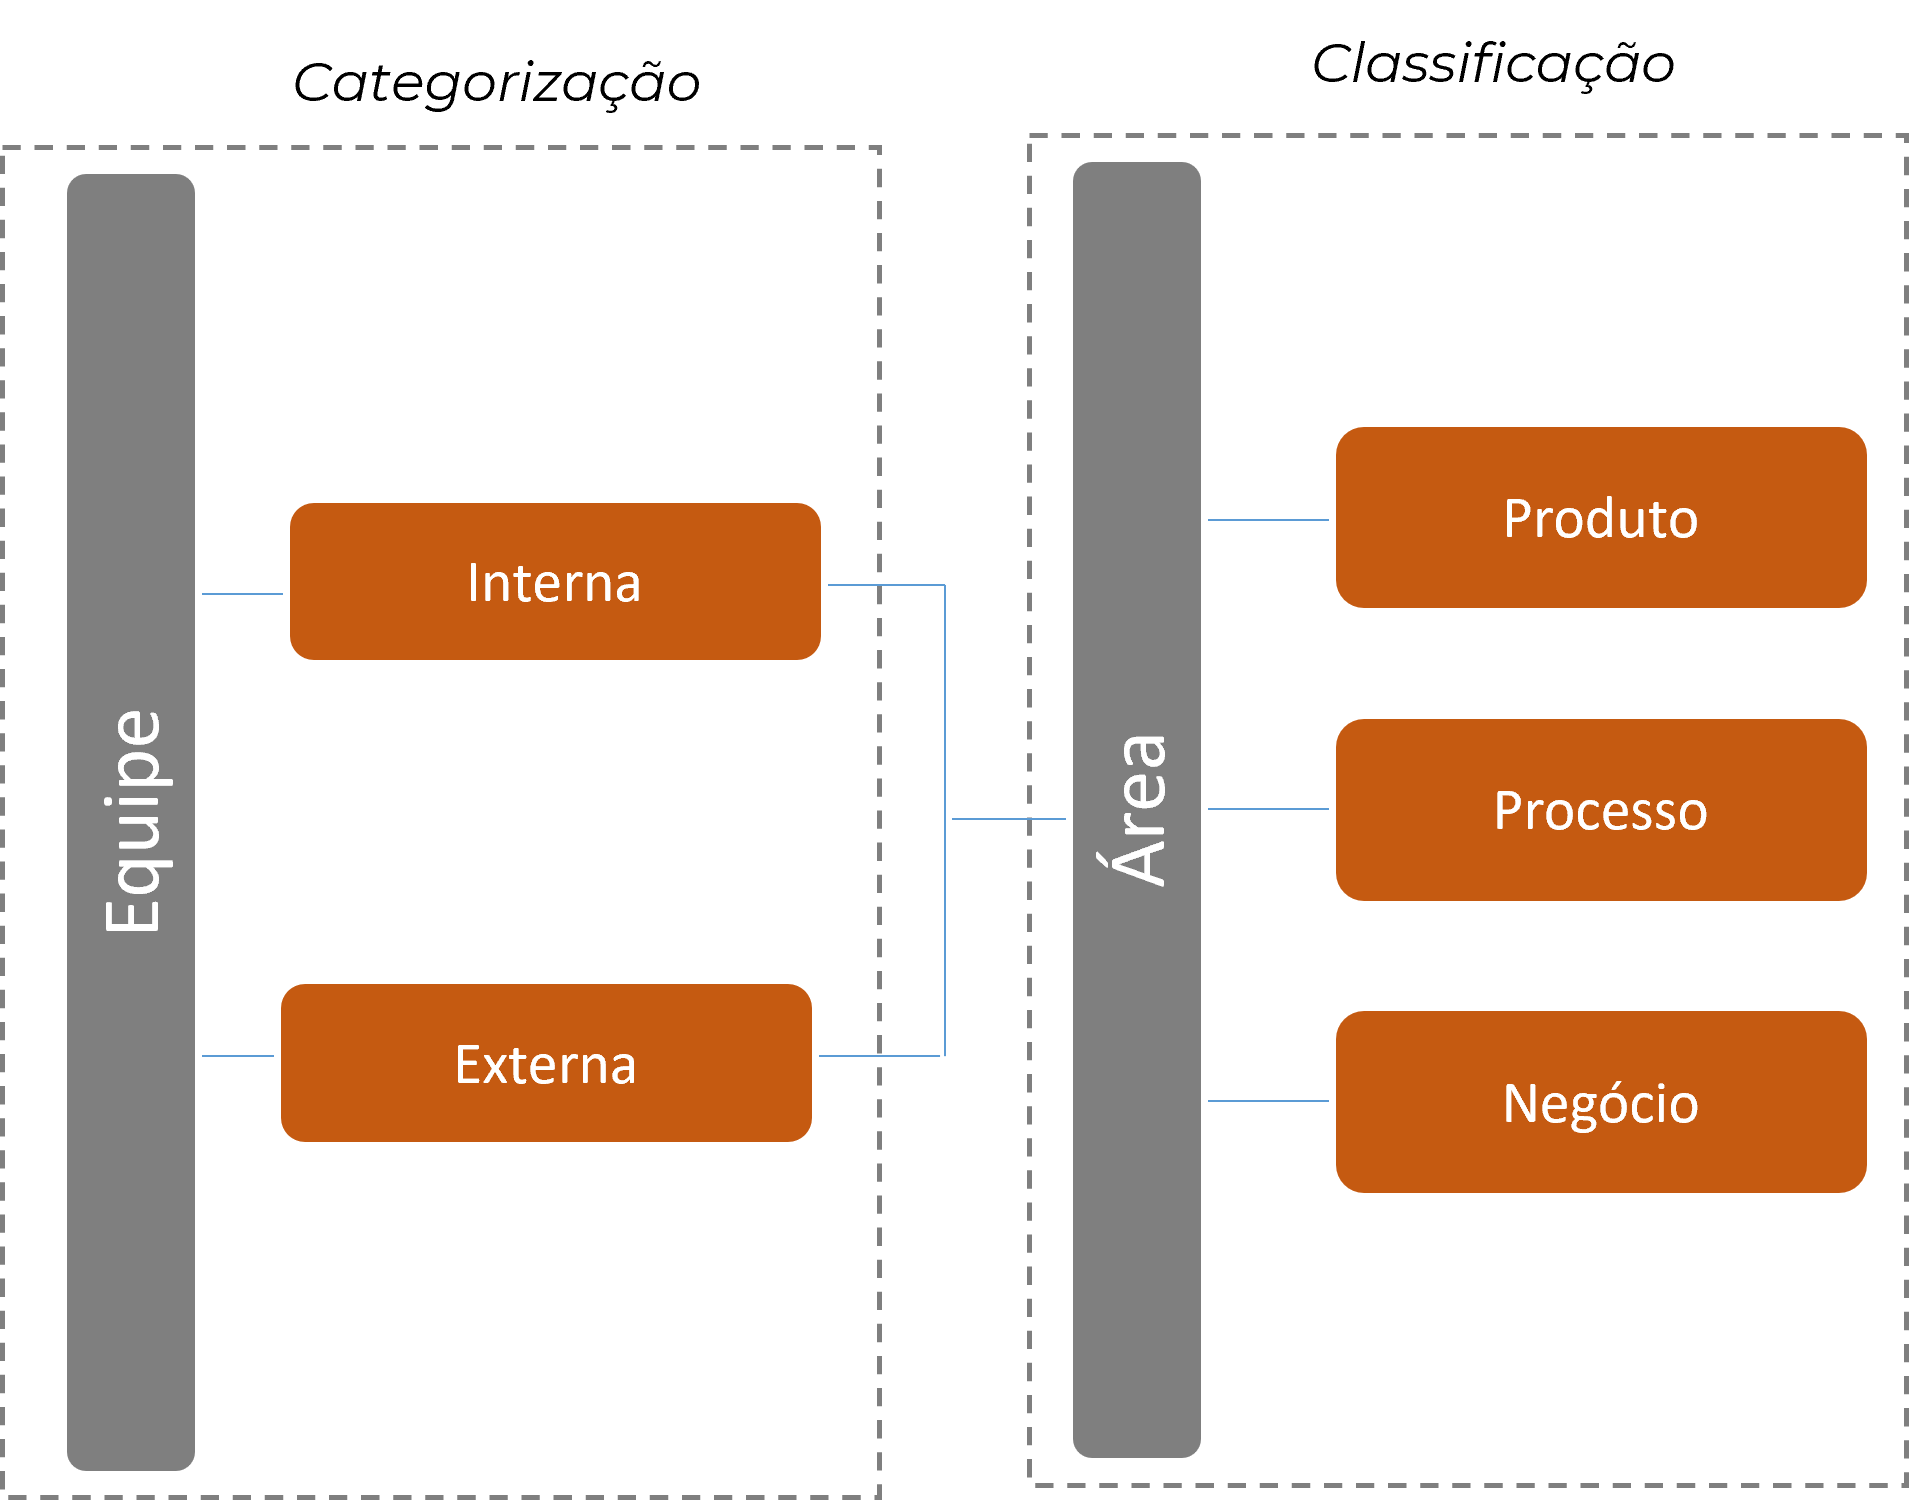
\includegraphics[width=0.7\textwidth]{entrevistados_area.png}
	
	Fonte: Elaborado pela Testing Company
\end{figure}

Por fim, as dores são classificadas em níveis de 1 (um) a 5 (cinco), envolvendo a gravidade e a tendência de impacto de uma situação, pode-se apoiar a priorizar problemas e oportunidades. 

 \begin{itemize}
	\item \textbf{Gravidade:} Refere-se ao impacto que o problema ou oportunidade pode causar se não for solucionado ou aproveitado, respectivamente. A gravidade pode ser classificada em cinco níveis:
	
	 \begin{itemize}
	 	\item Sem Gravidade: O problema ou oportunidade não tem impacto significativo.
	 	\item Pouco Grave: O problema ou oportunidade tem um impacto leve, que pode ser facilmente gerenciado.
	 	\item Grave: O problema ou oportunidade tem um impacto moderado, que pode exigir algum esforço para ser solucionado ou aproveitado.
	 	\item Muito Grave: O problema ou oportunidade tem um impacto significativo, que pode exigir recursos consideráveis para ser solucionado ou aproveitado.
	 	\item Extremamente Grave: O problema ou oportunidade tem um impacto crítico, que pode causar danos.
	 \end{itemize}
	 	
	\item \textbf{Tendência de Impacto: }Refere-se à probabilidade de o problema ou oportunidade se agravar com o tempo se nenhuma ação for tomada. A tendência de impacto pode ser classificada em três níveis:

	\begin{itemize}
		\item Tende a não piorar: O problema ou oportunidade não tende a se agravar com o tempo.
		\item Pode piorar a longo prazo: O problema ou oportunidade pode se agravar com o tempo, mas não de forma imediata.
		\item Pode piorar a médio prazo: O problema ou oportunidade pode se agravar com o tempo em um prazo moderado.
		\item Pode piorar em curto prazo: O problema ou oportunidade pode se agravar com o tempo em um prazo curto.
		\item Agravamento imediato: O problema ou oportunidade pode se agravar imediatamente, causando danos graves.
		
	\end{itemize}
\end{itemize}

\begin{figure}[H]
	\centering
	\caption{Matriz de Gravidade e Tendência de Impacto }
	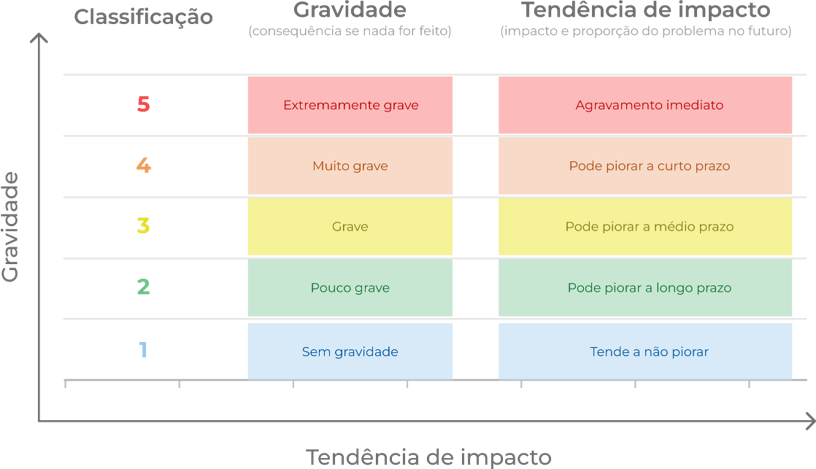
\includegraphics[width=0.7\textwidth]{matriz.png}
	
	Fonte: Elaborado pela Testing Company
\end{figure}

    

% =========================
% Resultados
% =========================
\chapter{Apresentação de Resultados}

\section{Contextualização do Processo Existente}

Embora a ALS Global seja uma grande organização, se olharmos para a quantidade de funcionários, o trabalho da consultoria está voltado a uma equipe menor, se não contarmos com as empresas terceiras. A equipe deve contar com algo entre 6 e 7 membros, no qual temos atribuições como, suporte, projetos, integrações, desenvolvimento, PO e direção. A poucos sistemas envolvidos também, o foco maior acaba sendo o S360. Esse sistema, por sua vez, surgiu no brasil e a ALS adquiriu o software. Esse produto, apesar de ter seus BUGs, possui um potencial de crescer para outros laboratórios dos quais ainda não está presente, visto que a ALS é um laboratório australiano que foi adquirindo vários outros laboratórios. A ALS Brasil é responsável pela operação da américa latina e da Europa. Já austrália, com outro sistema, é responsável pelo restante da operação. 

No geral, são feitas análises em óleo de motor, que passa por uma máquina, é feito análise (em média, para uma amostra são feitas 170 análises). Alguns casos as interpretações são feitas por IA, sem necessidade de um químico, já em outros casos podem ser solicitado pelo cliente a análise de um químico. Um ponto de atenção é que o sistema possui zero teste atualmente no código e majoritariamente hoje, a concentração de problemas são as alterações e melhorias feitas no sistema nos anos anteriores. Por fim, o sistema é um monolito feito em Angular JS e Grails, hospedado no Azure.

O modelo de trabalho atual presente na equipe é híbrido, em que o desenvolvimento é parcialmente interno e também terceirizado. De forma geral, as demandas podem surgir de várias origens diferentes, algumas a partir do suporte e outras a partir da direção. Olhando para o fluxo em que as demandas são oriundas do suporte, os clientes podem realizar suas solicitações através do envio de e-mails. Atualmente, os e-mails recebidos são automaticamente criados como tickets em uma ferramenta denominada de Manage Engine, o detalhe aqui é que os e-mails não obrigam que o ticket tenha detalhes ou outras informações, neste caso pode ocorrer que alguns chamados possuam um detalhamento menor por parte do cliente. 

Os tickets possuem um SLA para retorno de 24 horas, sendo assim, o suporte avalia se a situação é um problema, dúvida, melhoria e etc. Sendo um defeito ou melhoria isso é passado para desenvolvimento, no qual um item de trabalho é aberto no Azure Devops e posteriormente avaliado, detalhado e priorizado pela PO. Ressalta-se que existem grupos no Microsoft Teams que podem solicitar priorização, entretanto esses grupos podem acabar gerando alguns pontos de atenção, como solicitações de priorização sobre itens que visualmente não parecem ser tão prioritários.

Alternativamente, demandas podem ser oriundas da direção, que as encaminha por e-mail. Essas, por sua vez, são acompanhadas via Microsoft Planner e pelo Azure Devops. Também são detalhadas, priorizadas, passam por um entendimento técnico de um desenvolvedor da ALS Global e posteriormente são alocadas. As tarefas podem ser alocadas tanto na equipe interna quando com terceiros, entretanto, normalmente melhorias acabam indo para terceiros. As demandas ao serem passadas para uma empresa terceira, a mesma define prazo e precificação que é avaliada pela ALS Global e, se aprovado, segue-se para desenvolvimento. O desenvolvimento dos terceiros passa por um processo de code review pelo desenvolvedor da ALS Global e posteriormente é homologado internamente. Por fim é publicado em produção.

\begin{figure}[H]
	\centering
	\caption{Fluxograma}
	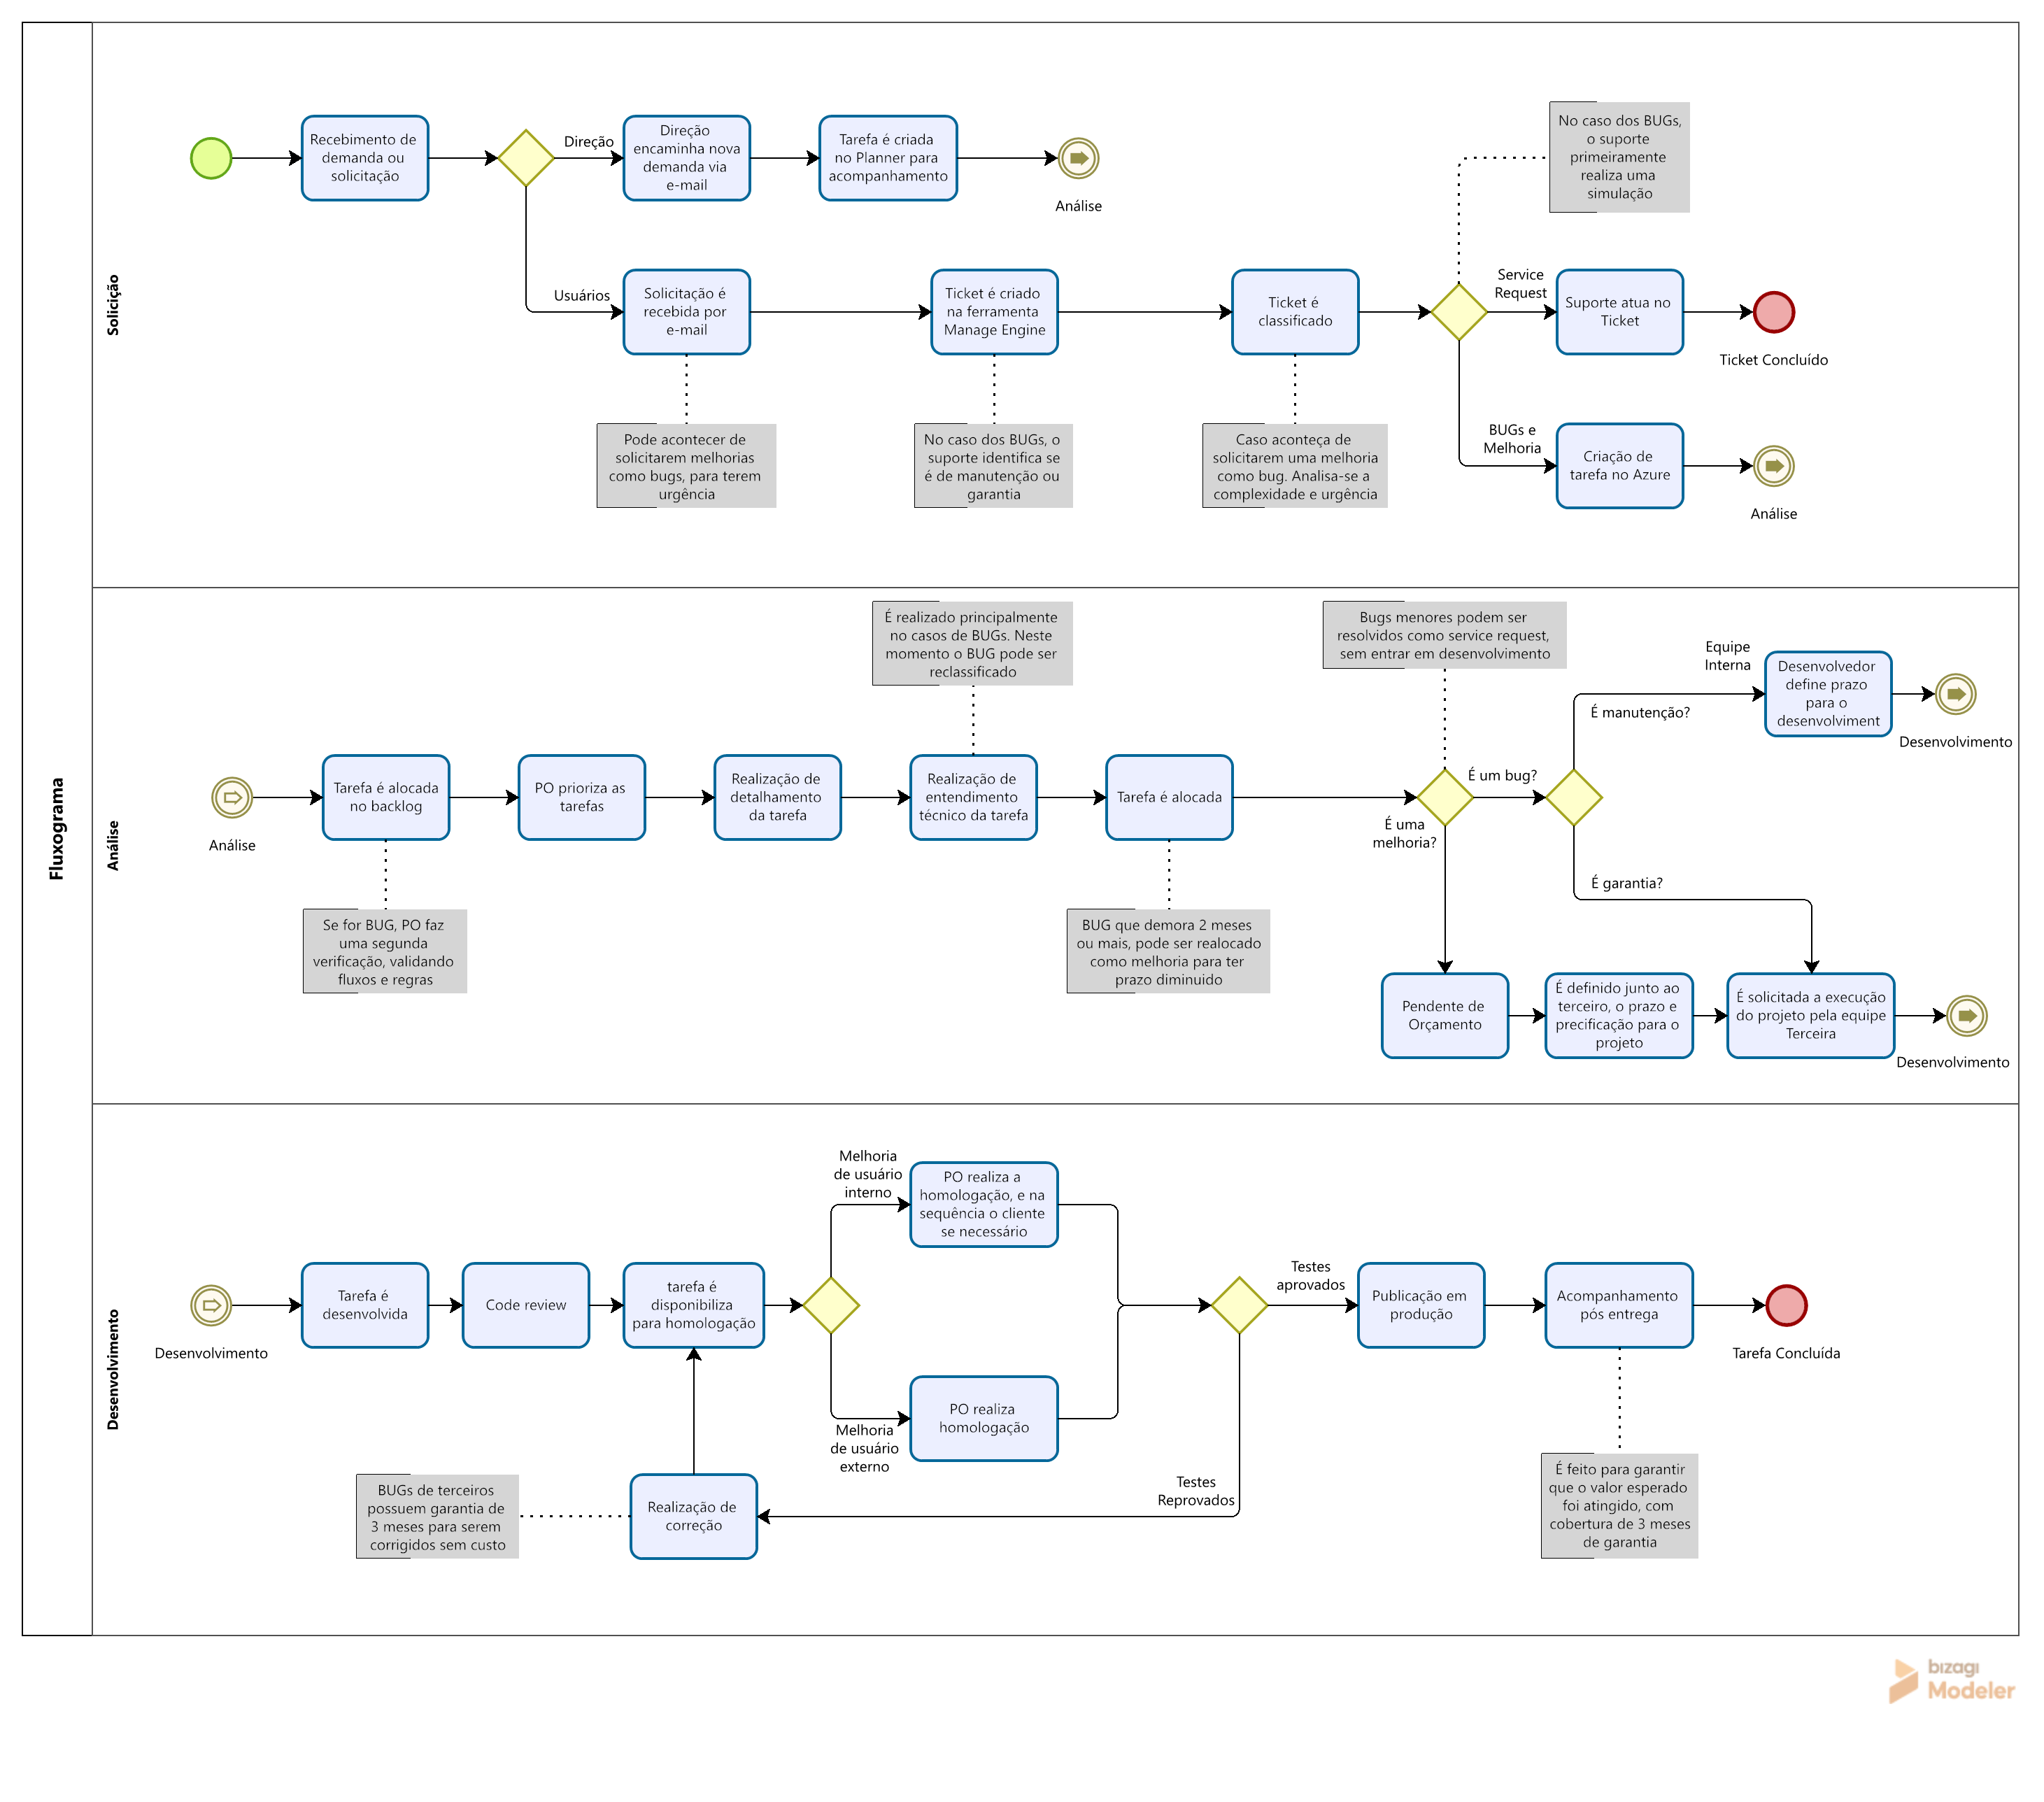
\includegraphics[width=1\textwidth]{Fluxograma.png}
	Fonte: Elaborado pela Testing Company
\end{figure}
     

\section{Dados do Questionário}

O questionário de colaboradores contou com a participação de seis profissionais, já o questionário direcionado aos terceiros contou com doze respostas. As perguntas abordaram diferentes aspectos, como tempo de empresa, fluxo de trabalho, pontos positivos, pontos negativos e entre outros.

\subsection{Sessão Dados do Profissional}

Nesta sessão, especialmente no questionário direcionado aos colaboradores, foram apresentadas perguntas relacionadas ao tempo de empresa e função exercida. O questionário dos colaboradores terceiros contou questões como fornecedor, nome do profissional e função exercida.


\subsection{Questionário de Colaboradores}

Os colaboradores da ALS Global descreveram seus fluxos de trabalho, com algumas exceções, de forma detalhada e com responsabilidades mistas. As atividades envolvem, por exemplo, suporte, desenvolvimento, acompanhamento de projetos, detalhamento de tarefas, priorização, validação e assim por diante. Alguns pontos positivos foram levantados pelos colaboradores, como a proximidade com o time e stakeholders, a organização das demandas no azure, a existência de um canal formal de atendimento via tickets e entre outros. A comunicação entre o time interno da ALS Global foi classificada entre 4 e 5, o que podemos entender como boa. Já a comunicação com as equipes terceiras às respostas variaram entre 3 e 5.

\begin{figure}[H]
	\vspace{1\baselineskip}
	\centering
	\caption{Questionário (Comunicação)}
	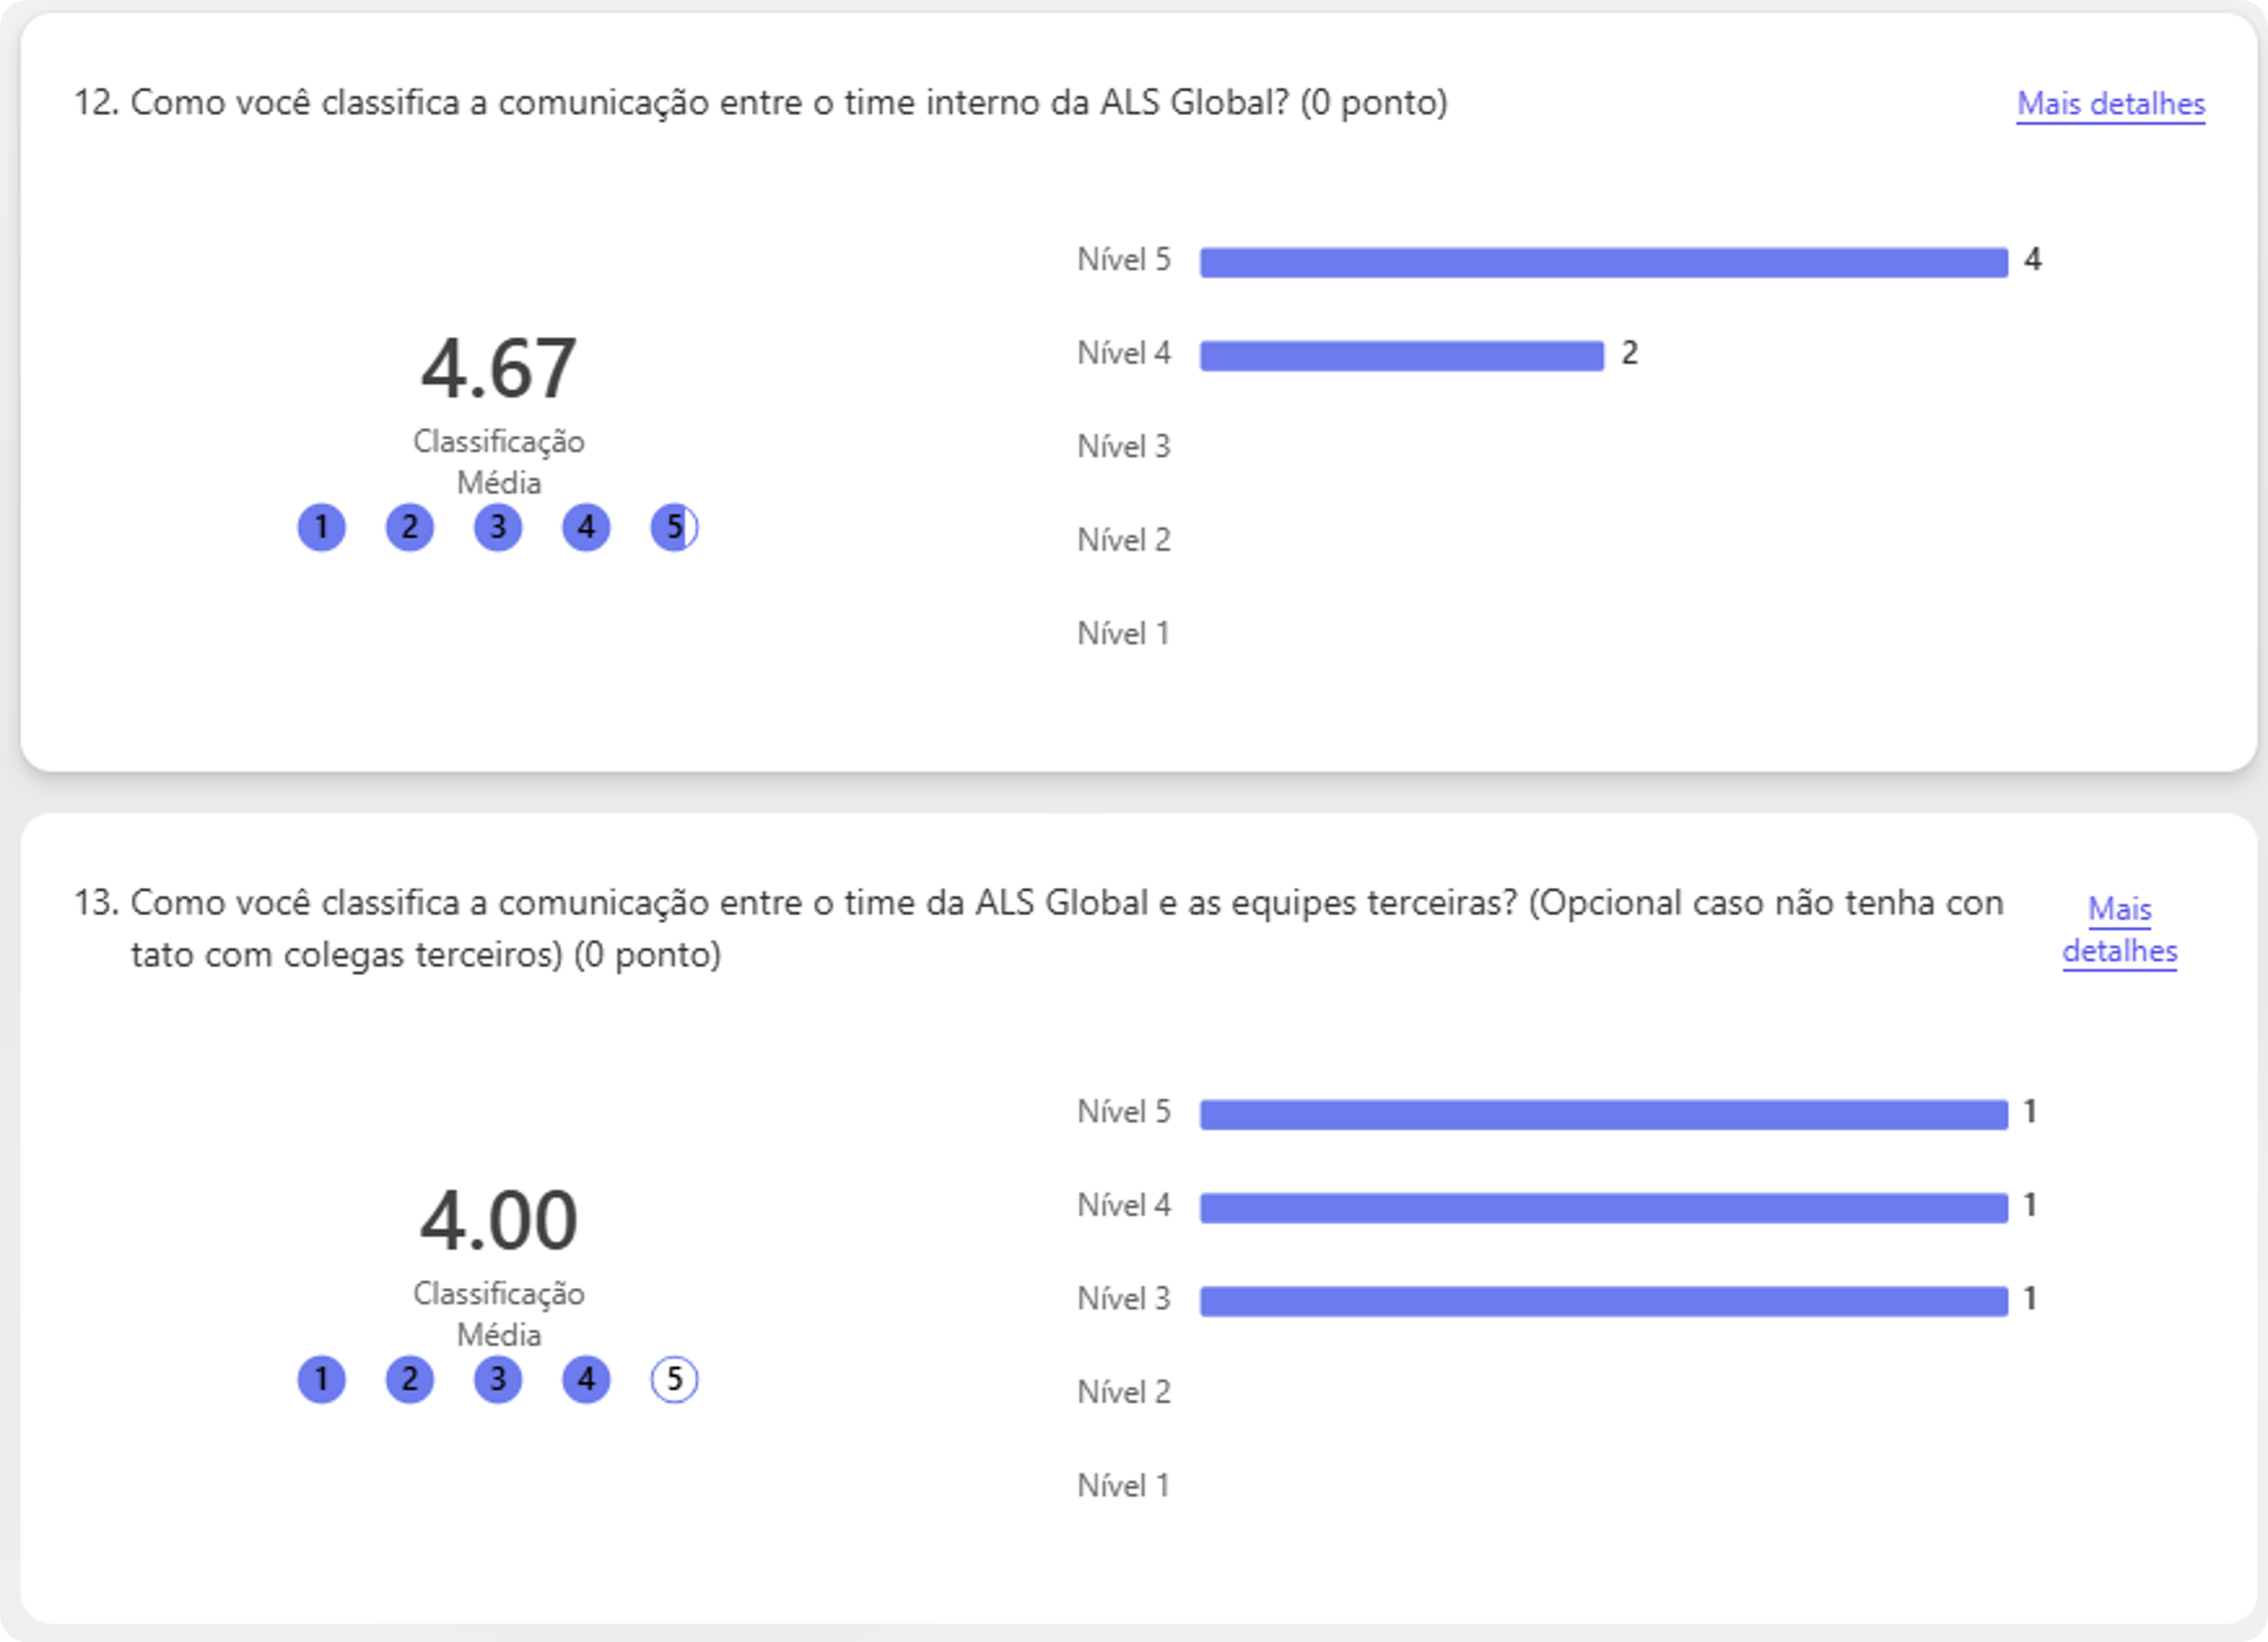
\includegraphics[width=0.85\textwidth]{form als comunicacao.png}
	
	Fonte: Elaborado pela Testing Company
\end{figure}


Pontos negativos também foram expostos pelos colaboradores internos, uma vez que essa questão foi abordada no questionário. Destacam-se, como exemplos, alto volume de demandas simultâneas, solicitações oriunda de canais paralelos aos tickets (Teams e WhatsApp), desalinhamento no fluxo entre áreas, onde usuários externos, por vezes, entram em contato direto com o time de TI sem abertura prévia de chamado. Adicionalmente pode-se trazer a qualidade das informações nos chamados recebidos, visto que os usuários conseguem abrir tickets de forma livre (modelo similar a e-mail), o que resulta frequentemente em solicitações com descrições incompletas, ausência de evidências e falta de informações básicas, como o sistema envolvido ou o tipo da demanda. Além desses pontos, também surgiu como ponto negativo o time ter parado de realizar dailies, a questão de respostas ao usuário, no qual é necessário informar sobre as atualizações dos chamados ou a falta delas. O acumulo de tarefas devido ao desenvolvedor interno necessitar lidar com tarefas de grande porte nas manutenções e também a possibilidade de estabelecer melhor os objetivos e requerimentos para desenvolvimento de automações de IA também surgiram.

Sobre a observação da equipe em relação a qualidade do produto e processo, muitas vezes uma ação no sistema acaba causando outros bugs, atualmente também o sistema possui 0\% de cobertura de testes, isso é complicado principalmente em um sistema com muito código deprecated e vários débitos técnicos. Dentre outros pontos, pode-se trazer aqui a questão de que a qualidade do processo pode estar sendo impactada pela pressão dos clientes e o volume de manutenções, assim como pode um ponto de melhoria a padronização de processos, usabilidade e redução de falhas recorrentes, visando maior eficiência operacional.

Abordando as melhorias que podem ocorrer no fluxo de trabalho dos fornecedores, pode-se trazer questões como comunicação, definição de prazos, transparência no andamento das demandas, melhoria nos testes e falta de comunicação sobre dúvidas ou questionamentos em casos de não entendimento claro das tarefas. sobre as ferramentas de trabalhado dispostas pela ALS Global, todas as avaliações estiveram acima de 3 na escala likert. Entretanto, existem políticas que impedem a equipe de testar novas ferramentas, visto que o sistema operacional é bloqueado para instalações e a empresa possui um escopo voltado a Microsoft. 

\subsection{Questionário de Terceiros}

Partindo para o questionário das equipes terceiras, o nível de detalhamento das tarefas e a clareza dos critérios de aceite possuem respostas variadas, mas destaca-se duas respostas que levantaram pontos interessantes. Em uma foi exposto que as propostas não apresentam um nível de escopo suficientemente claro, sendo necessárias diversas validações junto ao PO. Adicionalmente expõem aqui, embora a respota seja de uma profissional que atue antes do desenvolvimento, que as demandas não possuem critérios de aceite e regras de negócio totalmente definidos. Em alguns casos, o detalhamento poderia ser mais estruturado, o que demanda alinhamentos adicionais para garantir o entendimento completo antes do desenvolvimento.

Do ponto de vista das equipes terceiras, em algumas situações é necessário contato com a equipe da ALS Global. Adicionalmente, é observado em algumas poucas respostas que existe retrabalho por falta de alinhamento, mudança de escopo ou entendimento incompleto da demanda. Destaca-se duas no qual é indicado em uma que isso ocorre em praticamente todos os projetos, em quase todas as sprints, já em outra, é exposto que o retrabalho ocorre com certa frequência, principalmente devido a mudanças de escopo e ajustes após etapas já avançadas e validadas do processo, como definição e estruturação devidamente documentados. 

Sobre os principais fatores que dificultam, atrasam a execução das tarefas ou impactam sua produtividade no projeto, pontua-se a falta de clareza no escopo e ausência de refatorações/melhorias, já que novas funcionalidades são constantemente priorizadas e, embora essa respota seja de uma profissional que atue antes do desenvolvimento, a falta de definição clara de regras de negócio e critérios de aceite desde o início, além de mudanças de escopo ao longo do desenvolvimento. Dentro outras respotas em algumas perguntas, expõem-se aqui que uma das empresa indica, na questão sobre se o feedback recebido sobre as entregas costuma ser claro e útil para evolução do trabalho, que atualmente, não há clareza nesse ponto, e percebem que se pode evoluir para um modelo mais direcionado por projeto, considerando as particularidades de cada um e o volume de iniciativas em andamento. Ressalta-se que além dos itens trazidos ao presente relatório, mais pontos estão presentes nos questionários. Abaixo segue um gráfico extraído do Microsoft Forms referente a execução de algum tipo de teste no fluxo de trabalho.

\begin{figure}[H]
	\vspace{1\baselineskip}
	\centering
	\caption{Questionário (No seu fluxo de trabalho, é executado algum tipo de teste?)}
	\fbox{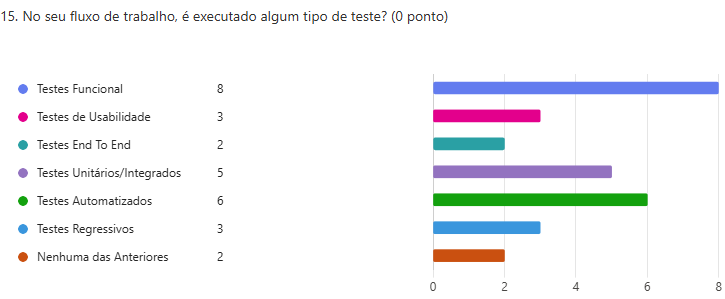
\includegraphics[width=1\textwidth]{form als 15.png}}
	
	Fonte: Elaborado pela Testing Company
\end{figure}


\section{Dores e Pontos de Atenção}

Finalizado os questionários e conversas individuais, compilou-se parte das informações coletadas para geração de um entregável contendo os principais problemas e oportunidades de melhoria reportados. Para isso, dividiu-se as dores selecionadas em: Contextualização Inicial, Entrevistas, Questionários (Colaboradores) e Questionários (Terceiros). As mesmas receberam uma categorização entre produto, processo ou negócio e um valor entre um e cinco para a gravidade e tendência de impactoo. Totalizaram mais de 120 pontos de dores, oportunidade de melhoria ou pontos de atenção. A seguir, são apresentadas algumas das dores, ressalta-se que os itens podem ser consultados na planilha disponibilizada pela consultoria.


\begin{figure}[H]
	\centering
	\caption{Parte das Dores e Pontos de Atenção (Contextualização Inicial)
	 }
	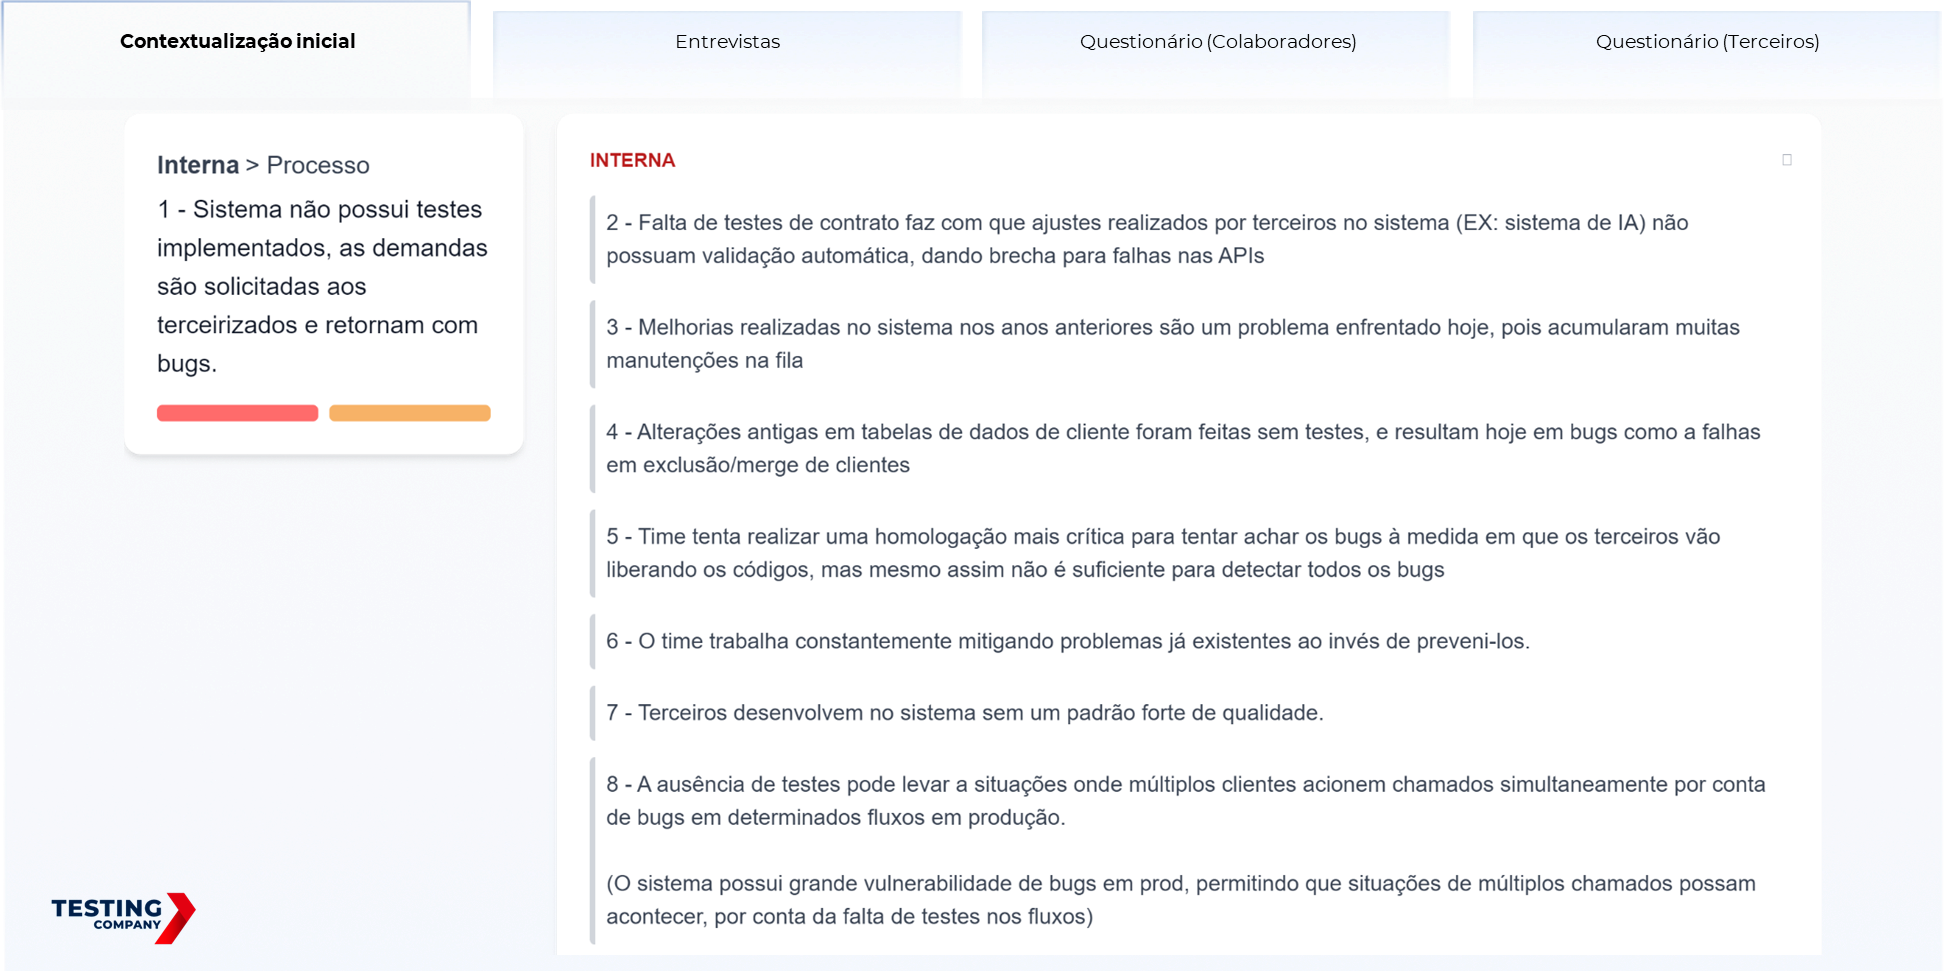
\includegraphics[width=1\textwidth]{Dores - Contextualização.png}
	
	Fonte: Elaborado pela Testing Company
\end{figure}

\begin{figure}[H]
	\centering
	\caption{Parte das Dores e Pontos de Atenção (Entrevistas)
	}
	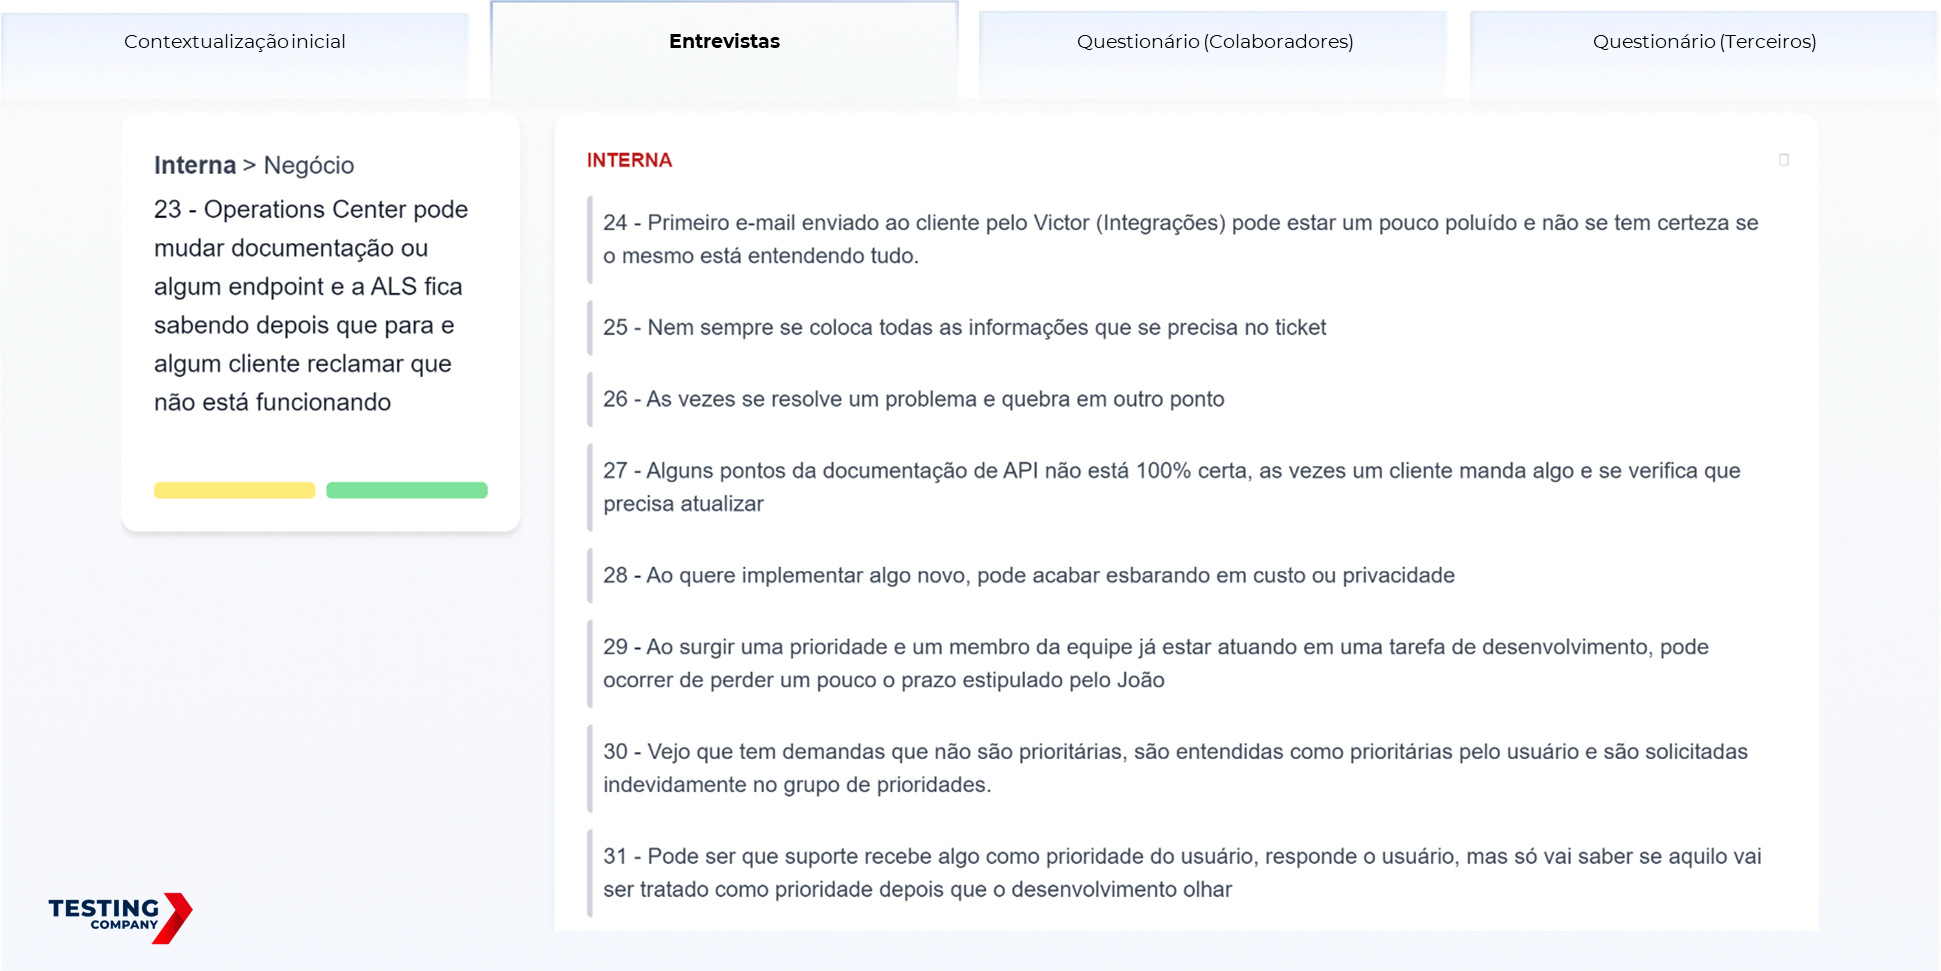
\includegraphics[width=1\textwidth]{Dores - Entrevistas.png}
	
	Fonte: Elaborado pela Testing Company
\end{figure}

\begin{figure}[H]
	\centering
	\caption{Parte das Dores e Pontos de Atenção (Questionário - Colaboradores)
	}
	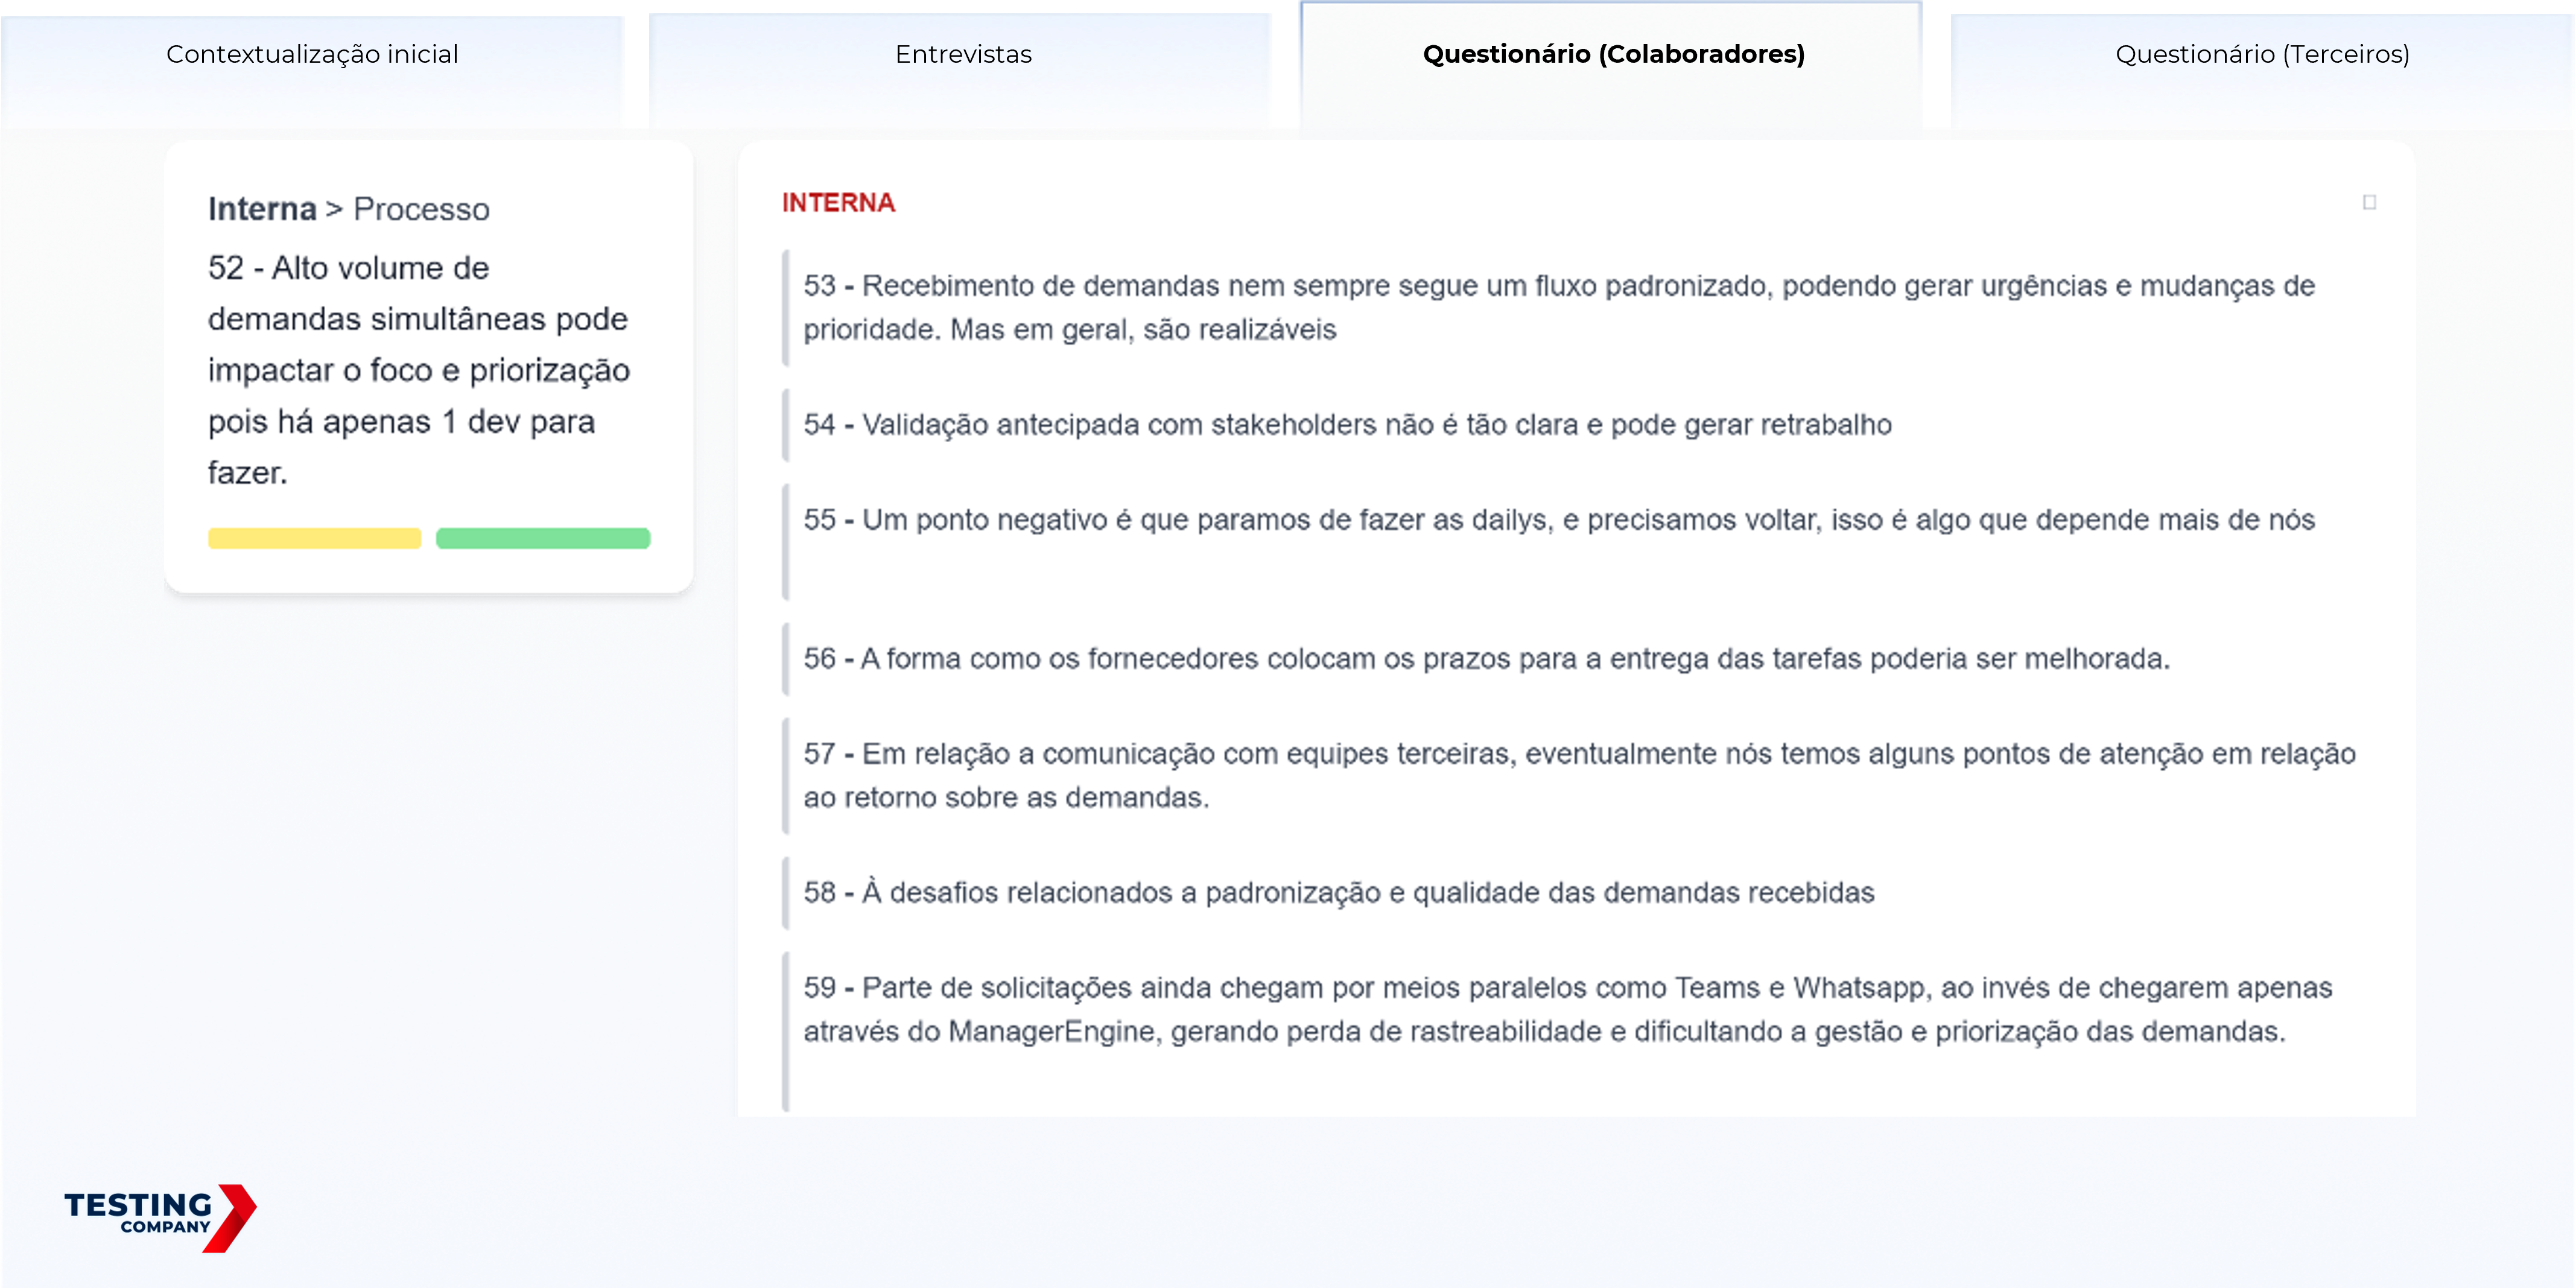
\includegraphics[width=1\textwidth]{Dores - Colaboradores.png}
	
	Fonte: Elaborado pela Testing Company
\end{figure}

\begin{figure}[H]
	\centering
	\caption{Parte das Dores e Pontos de Atenção (Questionário - Terceiros)
	}
	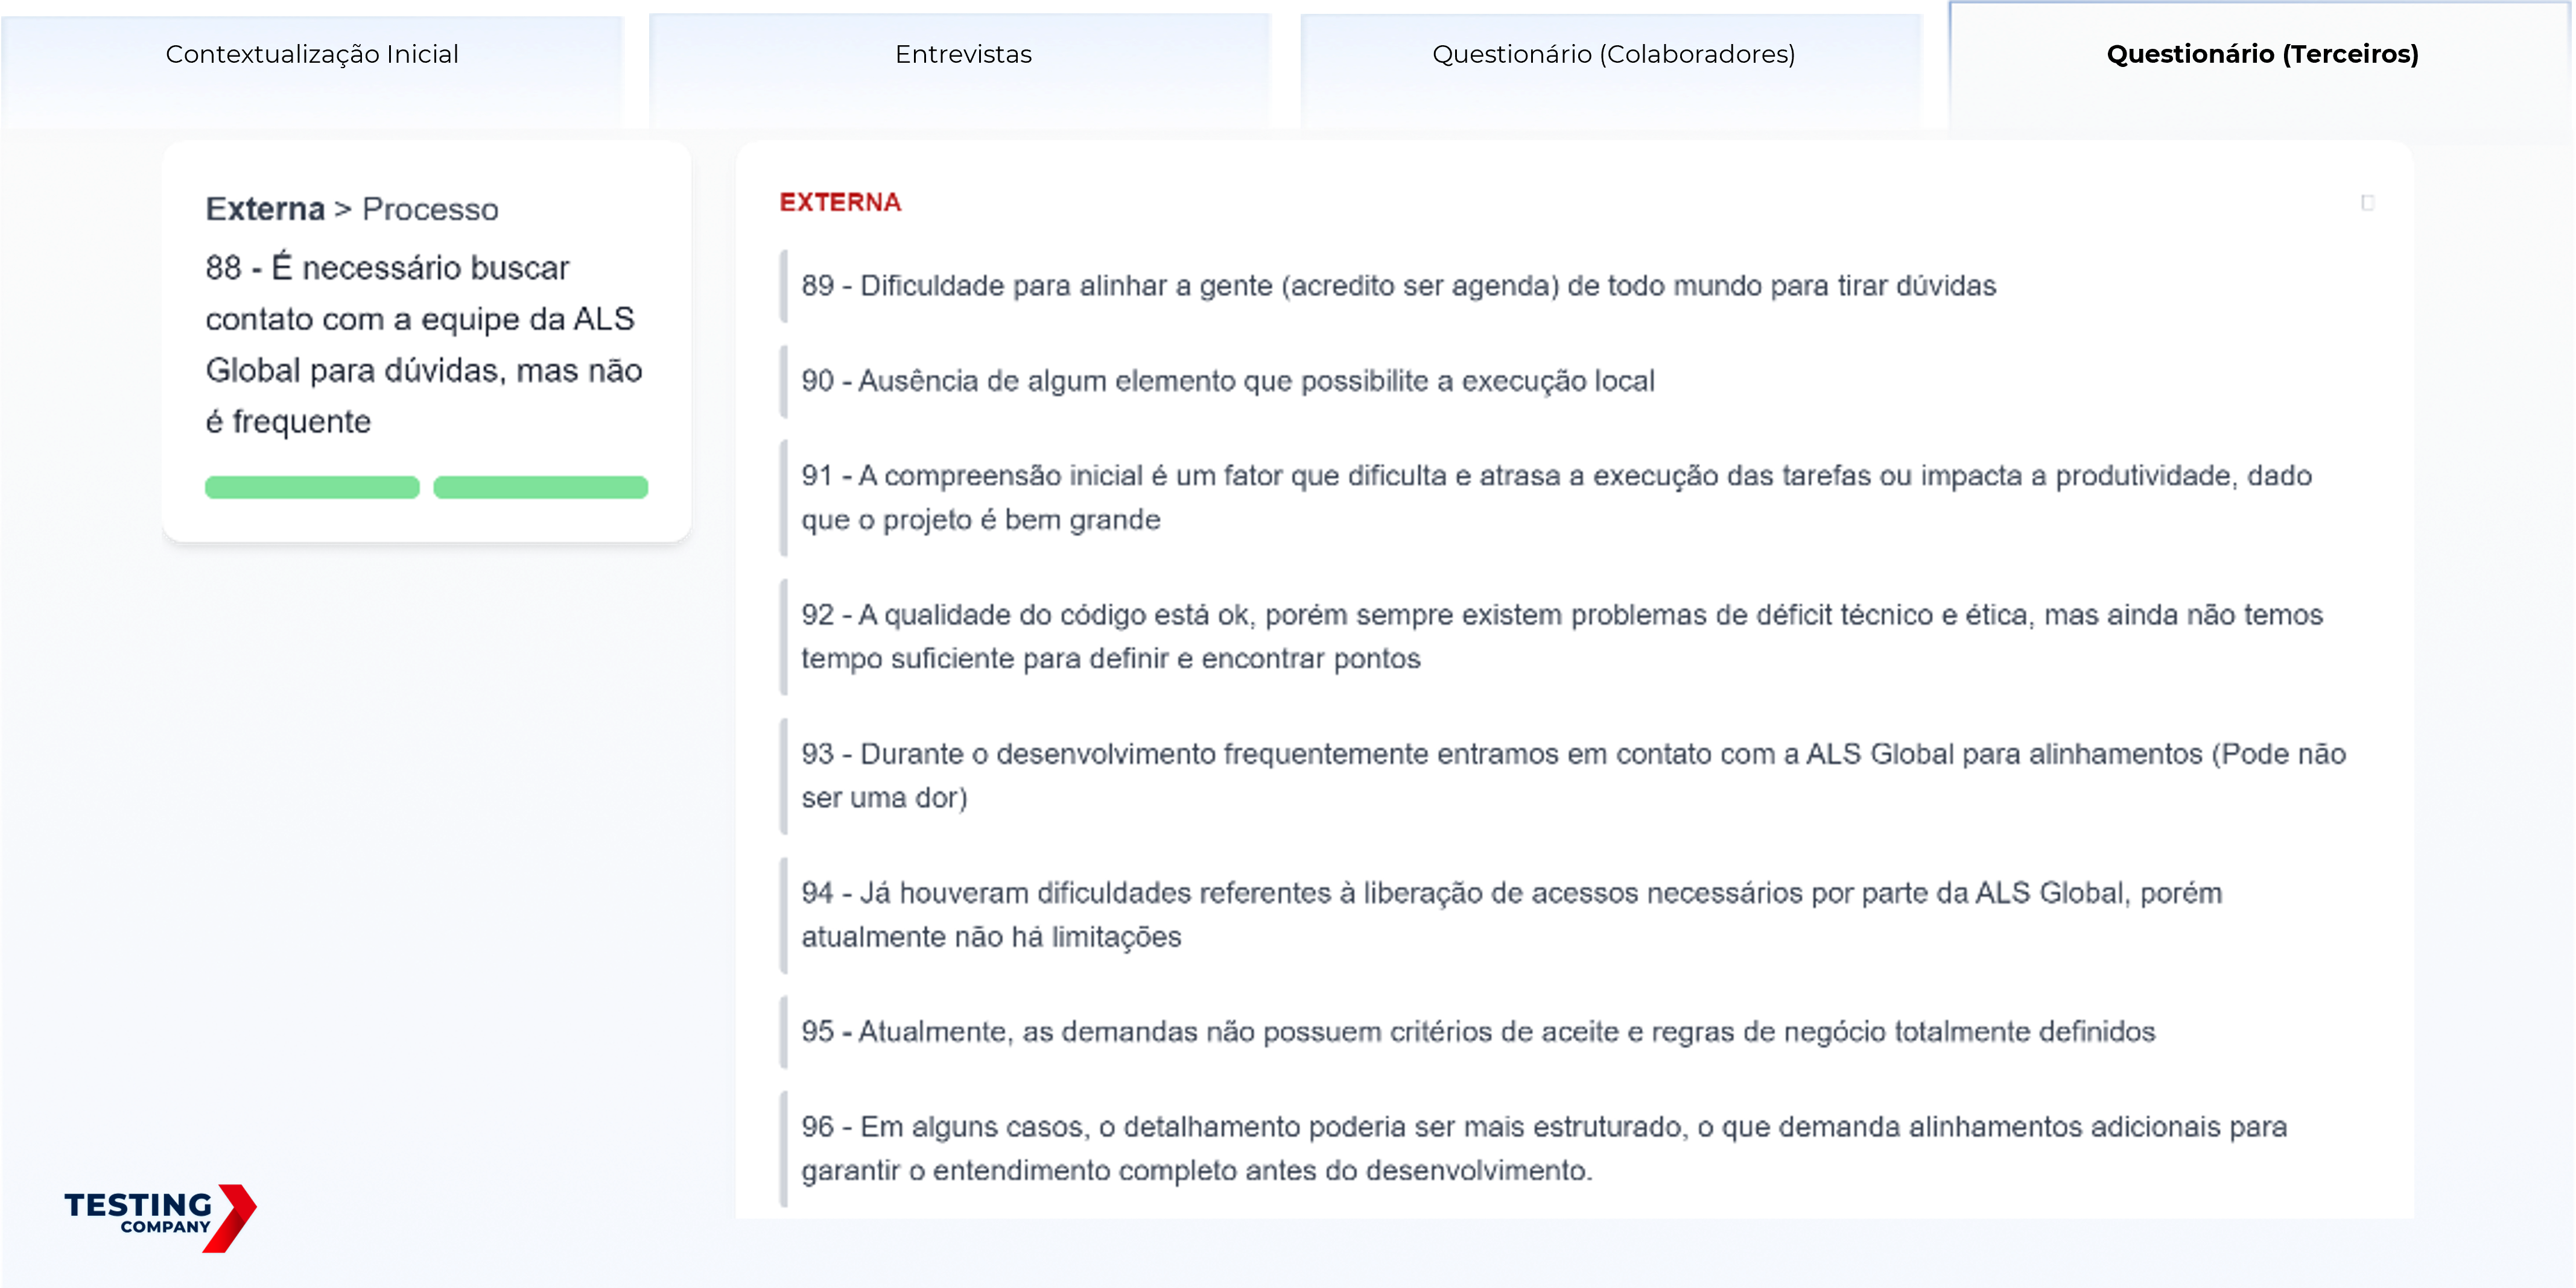
\includegraphics[width=1\textwidth]{Dores - Terceiros.png}
	
	Fonte: Elaborado pela Testing Company
\end{figure}
 

% =========================
% Nível de Maturidade
% =========================
\chapter{Nível de Maturidade Diagnosticado}

Neste documento, mais especificamente no tópico 4 (quatro), foi exposto algumas informações referentes ao plano da qualidade, o modelo que auxilia no diagnóstico do nível de maturidade. Ressalta-se que o modelo é dividido em 5 (cinco) níveis, sendo eles estágios de evolução que apoiam nas discussões sobre o que pode ser melhorado e/ou evoluído. 

A realização de conversas individuais em conjunto com a aplicação do questionário permitiu que os próprios profissionais expusessem aspectos positivos e negativos sobre organização. Foram coletados alguns pontos de melhoria e pontos de atenção que somaram mais de 120 itens. Ressalta-se que a empresa já conta, por exemplo, com testes na etapa de homologação, conduzidos pela PO e, quando necessário, pelo cliente e possui a prática de documentar os defeitos identificados, esses registros apoiam no acompanhamento dos problemas reportados pelos usuários.

Entretanto, mesmo com alguns processos de teste e desenvolvimento, há também aspectos que podem ser evoluídos. A automação de testes, por exemplo, ainda não está presente no fluxo de trabalho da equipe e os testes manuais realizados pelos terceiros ainda possuem oportunidades de melhoria. Por fim, entende-se que apesar da existência de alguns processos de teste a maturidade do fluxo de trabalho atual segue classificada como nível \textbf{Nível 1 – Inicial}.

\begin{figure}[H]
	\centering
	\caption{Nível de Maturidade
	 }
	
\includegraphics[width=0.2\textwidth]{Jornada da Qualidade/1.inicial.png}
	
	Fonte: Elaborado pela Testing Company
\end{figure}


 \PaginaFinalImagem{ultima_imagem.png}


\end{document}